%!TEX TS-program = xelatex
\documentclass[11pt]{article}

\usepackage[english]{babel}

\usepackage{amsmath,amssymb,amsfonts}
\usepackage[utf8]{inputenc}
\usepackage[T1]{fontenc}
\usepackage{stix}
\usepackage[scaled]{helvet}
\usepackage[scaled]{inconsolata}

\usepackage{lastpage}

\usepackage{setspace}

\usepackage{ccicons}

\usepackage[hang,flushmargin]{footmisc}

\usepackage{geometry}

\setlength{\parindent}{0pt}
\setlength{\parskip}{6pt plus 2pt minus 1pt}

\usepackage{fancyhdr}
\renewcommand{\headrulewidth}{0pt}\providecommand{\tightlist}{%
  \setlength{\itemsep}{0pt}\setlength{\parskip}{0pt}}

\makeatletter
\newcounter{tableno}
\newenvironment{tablenos:no-prefix-table-caption}{
  \caption@ifcompatibility{}{
    \let\oldthetable\thetable
    \let\oldtheHtable\theHtable
    \renewcommand{\thetable}{tableno:\thetableno}
    \renewcommand{\theHtable}{tableno:\thetableno}
    \stepcounter{tableno}
    \captionsetup{labelformat=empty}
  }
}{
  \caption@ifcompatibility{}{
    \captionsetup{labelformat=default}
    \let\thetable\oldthetable
    \let\theHtable\oldtheHtable
    \addtocounter{table}{-1}
  }
}
\makeatother

\usepackage{array}
\newcommand{\PreserveBackslash}[1]{\let\temp=\\#1\let\\=\temp}
\let\PBS=\PreserveBackslash

\usepackage[breaklinks=true]{hyperref}
\hypersetup{colorlinks,%
citecolor=blue,%
filecolor=blue,%
linkcolor=blue,%
urlcolor=blue}
\usepackage{url}

\usepackage{caption}
\setcounter{secnumdepth}{0}
\usepackage{cleveref}

\usepackage{graphicx}
\makeatletter
\def\maxwidth{\ifdim\Gin@nat@width>\linewidth\linewidth
\else\Gin@nat@width\fi}
\makeatother
\let\Oldincludegraphics\includegraphics
\renewcommand{\includegraphics}[1]{\Oldincludegraphics[width=\maxwidth]{#1}}

\usepackage{longtable}
\usepackage{booktabs}

\usepackage{color}
\usepackage{fancyvrb}
\newcommand{\VerbBar}{|}
\newcommand{\VERB}{\Verb[commandchars=\\\{\}]}
\DefineVerbatimEnvironment{Highlighting}{Verbatim}{commandchars=\\\{\}}
% Add ',fontsize=\small' for more characters per line
\usepackage{framed}
\definecolor{shadecolor}{RGB}{248,248,248}
\newenvironment{Shaded}{\begin{snugshade}}{\end{snugshade}}
\newcommand{\KeywordTok}[1]{\textcolor[rgb]{0.13,0.29,0.53}{\textbf{#1}}}
\newcommand{\DataTypeTok}[1]{\textcolor[rgb]{0.13,0.29,0.53}{#1}}
\newcommand{\DecValTok}[1]{\textcolor[rgb]{0.00,0.00,0.81}{#1}}
\newcommand{\BaseNTok}[1]{\textcolor[rgb]{0.00,0.00,0.81}{#1}}
\newcommand{\FloatTok}[1]{\textcolor[rgb]{0.00,0.00,0.81}{#1}}
\newcommand{\ConstantTok}[1]{\textcolor[rgb]{0.00,0.00,0.00}{#1}}
\newcommand{\CharTok}[1]{\textcolor[rgb]{0.31,0.60,0.02}{#1}}
\newcommand{\SpecialCharTok}[1]{\textcolor[rgb]{0.00,0.00,0.00}{#1}}
\newcommand{\StringTok}[1]{\textcolor[rgb]{0.31,0.60,0.02}{#1}}
\newcommand{\VerbatimStringTok}[1]{\textcolor[rgb]{0.31,0.60,0.02}{#1}}
\newcommand{\SpecialStringTok}[1]{\textcolor[rgb]{0.31,0.60,0.02}{#1}}
\newcommand{\ImportTok}[1]{#1}
\newcommand{\CommentTok}[1]{\textcolor[rgb]{0.56,0.35,0.01}{\textit{#1}}}
\newcommand{\DocumentationTok}[1]{\textcolor[rgb]{0.56,0.35,0.01}{\textbf{\textit{#1}}}}
\newcommand{\AnnotationTok}[1]{\textcolor[rgb]{0.56,0.35,0.01}{\textbf{\textit{#1}}}}
\newcommand{\CommentVarTok}[1]{\textcolor[rgb]{0.56,0.35,0.01}{\textbf{\textit{#1}}}}
\newcommand{\OtherTok}[1]{\textcolor[rgb]{0.56,0.35,0.01}{#1}}
\newcommand{\FunctionTok}[1]{\textcolor[rgb]{0.00,0.00,0.00}{#1}}
\newcommand{\VariableTok}[1]{\textcolor[rgb]{0.00,0.00,0.00}{#1}}
\newcommand{\ControlFlowTok}[1]{\textcolor[rgb]{0.13,0.29,0.53}{\textbf{#1}}}
\newcommand{\OperatorTok}[1]{\textcolor[rgb]{0.81,0.36,0.00}{\textbf{#1}}}
\newcommand{\BuiltInTok}[1]{#1}
\newcommand{\ExtensionTok}[1]{#1}
\newcommand{\PreprocessorTok}[1]{\textcolor[rgb]{0.56,0.35,0.01}{\textit{#1}}}
\newcommand{\AttributeTok}[1]{\textcolor[rgb]{0.77,0.63,0.00}{#1}}
\newcommand{\RegionMarkerTok}[1]{#1}
\newcommand{\InformationTok}[1]{\textcolor[rgb]{0.56,0.35,0.01}{\textbf{\textit{#1}}}}
\newcommand{\WarningTok}[1]{\textcolor[rgb]{0.56,0.35,0.01}{\textbf{\textit{#1}}}}
\newcommand{\AlertTok}[1]{\textcolor[rgb]{0.94,0.16,0.16}{#1}}
\newcommand{\ErrorTok}[1]{\textcolor[rgb]{0.64,0.00,0.00}{\textbf{#1}}}
\newcommand{\NormalTok}[1]{#1}

\newlength{\cslhangindent}
\setlength{\cslhangindent}{1.5em}
\newlength{\csllabelwidth}
\setlength{\csllabelwidth}{3em}
\newenvironment{CSLReferences}[3] % #1 hanging-ident, #2 entry spacing
 {% don't indent paragraphs
  \setlength{\parindent}{0pt}
  % turn on hanging indent if param 1 is 1
  \ifodd #1 \everypar{\setlength{\hangindent}{\cslhangindent}}\ignorespaces\fi
  % set entry spacing
  \ifnum #2 > 0
  \setlength{\parskip}{#2\baselineskip}
  \fi
 }%
 {}
\usepackage{calc} % for \widthof, \maxof
\newcommand{\CSLBlock}[1]{#1\hfill\break}
\newcommand{\CSLLeftMargin}[1]{\parbox[t]{\maxof{\widthof{#1}}{\csllabelwidth}}{#1}}
\newcommand{\CSLRightInline}[1]{\parbox[t]{\linewidth}{#1}}
\newcommand{\CSLIndent}[1]{\hspace{\cslhangindent}#1}\geometry{verbose,letterpaper,tmargin=2.5cm,bmargin=2.5cm,lmargin=2.5cm,rmargin=4.5cm}

\usepackage{lineno}
\usepackage[nolists,noheads]{endfloat}

\pagestyle{plain}

\doublespacing

\fancypagestyle{normal}
{
  \fancyhf{}
  \fancyfoot[R]{\footnotesize\sffamily\thepage\ of \pageref*{LastPage}}
}
\begin{document}
\thispagestyle{empty}
{\Large\bfseries\sffamily A Roadmap Toward Prediction of Ecological
Networks Across Space and Time}
\vskip 5em

Tanya\,Strydom\,\textsuperscript{1,2}\quad Michael
David\,Catchen\,\textsuperscript{3,2}\quad Francis\,Banville\,\textsuperscript{1,4,2}\quad Dominique\,Caron\,\textsuperscript{3,2}\quad Gabriel\,Dansereau\,\textsuperscript{1,2}\quad Norma\,Forero\,\textsuperscript{1,2}\quad Gracielle\,Higino\,\textsuperscript{5}\quad Benjamin\,Mercier\,\textsuperscript{4,2}\quad Andrew\,Gonzalez\,\textsuperscript{3,2}\quad Laura\,Pollock\,\textsuperscript{3,2}\quad Timothée\,Poisot\,\textsuperscript{1,2,*}

\textsuperscript{1}\,Université de
Montréal\quad \textsuperscript{2}\,Québec Centre for Biodiversity
Sciences\quad \textsuperscript{3}\,McGill
University\quad \textsuperscript{4}\,Université de
Sherbrooke\quad \textsuperscript{5}\,Universidade Federal de Goiás

\textsuperscript{*}\,\,\texttt{timothee.poisot@umontreal.ca}

\vfill
This work is released by its authors under a CC-BY 4.0 license\hfill\ccby\\
Last revision: \emph{\today}

\clearpage
\thispagestyle{empty}

\vfill
\textbf{\sffamily Abstract: }Ecological networks can capture meaningful
information on the structure of ecological communities. Yet the scarcity
of existing data, and the difficulty associated with comprehesively
sampling ecological interactions, means that to describe the structure,
variation, and change of ecological networks over time and space, we
need to rely on modelling tools with the capacity to make accurate
predictions about how species interact. In this review, we offer a
roadmap aimed at guiding the development and integration of these tools,
with the specific purpose of boosting our predictive ability. By working
from first principles on the mechanisms involved in structuring
ecological networks, we make recommendations about the scale at which we
can predict networks across both biological organization as well as
space and time. In so doing, we show that multiple sources of data and
quantitative approaches, including statistical, dynamical, and
inferential models, can and must be integrated to deliver forecasts of
ecological networks. Importantly, we argue that ecological forecasting
applied to networks will provide benefits to other fields of ecology: it
will notably improve the integration between network ecology and
metacommunity theory and highlight the interoperability between
different data sources. Here, we take a question driven approach to
review our current understanding of ecological networks, sketch the path
forward for this research program.
\vfill

\clearpage
\linenumbers
\pagestyle{normal}

\hypertarget{introduction}{%
\section{Introduction}\label{introduction}}

Ecosystems \emph{are} interactions -- organisms interact with
one-another and with their environment, either directly or indirectly.
Between organisms, these interactions form networks of varying
complexity, drive ecological and evolutionary dynamics, and maintain
ecosystem diversity and functioning (Delmas et al. 2018; Landi et al.
2018; Albrecht et al. 2018). Networks of species interactions underpin
our understanding of key ecological processes (Pascual and Dunne 2006;
Heleno et al. 2014). Yet, even basic knowledge of species interactions
(like being able to list them, or guess which ones may exist) is one of
the most severe shortfalls in biodiversity science (Hortal et al. 2015).
This is due in large part to the tedious, time-consuming, and expensive
data collection process. As with many ecological systems, networks of
species interactions have entered their ``long now'' (Carpenter 2002),
where contemporary actions have long-term, low-predictability
consequences (Burkle, Marlin, and Knight 2013).

Therefore, our field needs a conceptual path forward toward models that
enable prediction (for the present) and forecasting (for the future) of
species interactions and the networks they form (McCann 2007; Seibold et
al. 2018). Here we provide a data-driven illustration to show how
machine learning approaches can enable unreasonably effective prediction
of interactions whereby we construct a metaweb of host-parasite
interactions across space, which serves as a proof-of-concept for this
conceptual framework. We then propose a roadmap forward for how to
improve predictions using this approach, and provide a primer on the
relevant tools and methods that could be incorporated into models of
this type in the future in order to account for the spatial, temporal,
and climatic dimensions of network prediction (Burkle and Alarcon 2011).

\hypertarget{proof-of-concept-can-we-predict-ecological-networks}{%
\section{Proof-of-Concept: can we predict ecological
networks?}\label{proof-of-concept-can-we-predict-ecological-networks}}

The core premise of this manuscript is that ecological networks can be
predicted. In this section, we provide a proof-of-concept, in which we
(i) aggregate a series of networks collected across space into a
metaweb, (ii) extract features based on species co-occurrence, (iii) use
these features to train a neural network to predict interactions, and
(iv) apply this classifier to the original features to predict possibly
missing interactions across the entire species pool. The entire analysis
is presented in fig.~\ref{fig:example}, and the code to reproduce it is
available at \textbf{TODO OSF LINK}; the entire example was carried out
in \emph{Julia 1.5.3} (Bezanson et al. 2017), and notably uses the
\emph{Flux} machine learning framework (Innes 2018). Note that this
analysis is meant to serve as an \emph{example only}, and should in
practice be fined-tuned according to the state of the art (\emph{e.g.}
Goodfellow, Bengio, and Courville 2016).

We used data from Hadfield et al. (2014), describing 51 host-parasite
networks, where not all species pairs co-occur across sites. This
implies that there are ``negative associations'' that might be
biologically feasible but not observed because the two species have not
been observed in co-occurrence. As this dataset has no features like
species traits on which to base a predictive model, we have aggregated
all interactions into a binary metaweb (J. Dunne 2006). We then
transformed the (undirected) metaweb through a probabilistic PCA
(Tipping and Bishop 1999), so as to create a number of latent features
for the species in a context where the dataset is both unbalanced and
likely to have many missing values. This frames the problem as
predicting a binary outcome, the interaction \(M_{xy}\) represented as
\texttt{true} or \texttt{false} based on a features vector
\(v_{xy} = [v_x, v_y]\) where \(v_x\) is the values of the selected
features for the parasite and \(v_y\) is the features of the host. In
the following example, we used the first 15 components of the latent
sub-space created by the probabilistic PCA. This features vector is then
fed into the input layer of a neural network, which uses three hidden
layers with appropriate dropout rates (\(0.5\)), and finally a
two-neurons output layer whose result is softmaxed to pick the most
likely outcome, \emph{i.e.} the interaction bit describing an
interaction when equal to 1, and no interaction when equal to 0.

\begin{figure}
\hypertarget{fig:example}{%
\centering
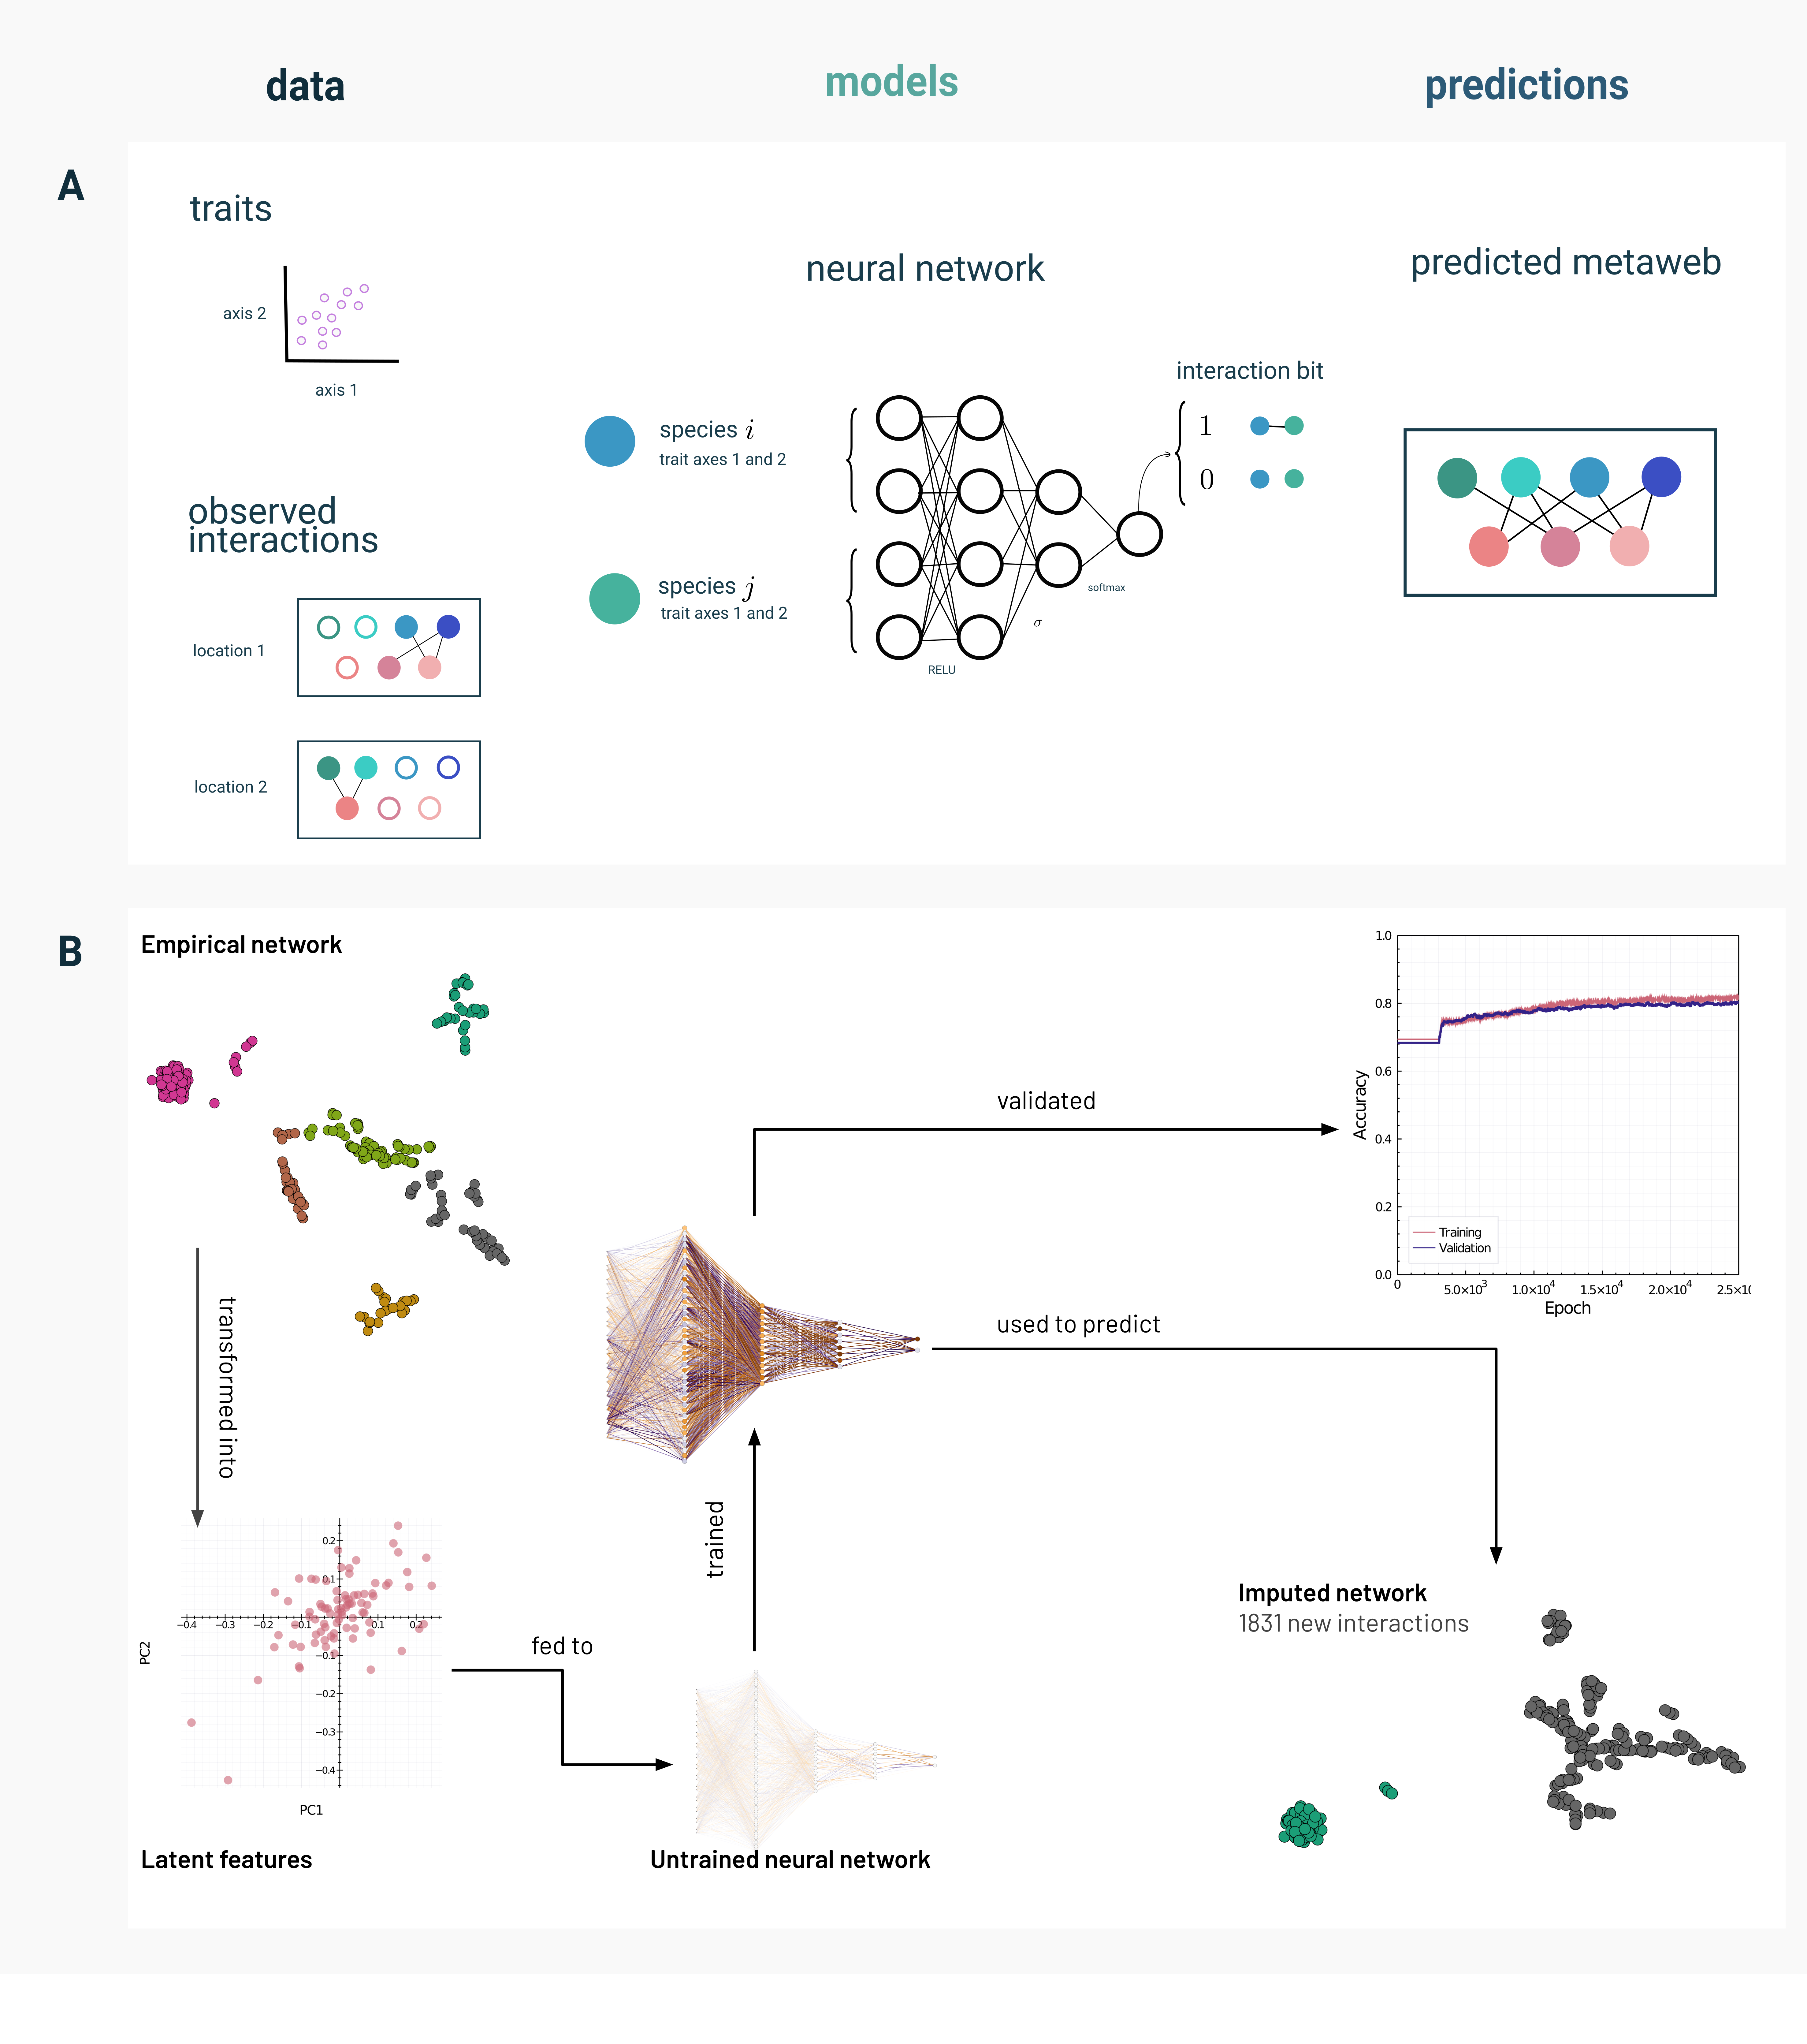
\includegraphics{figures/example_network_prediction.png}
\caption{(A) A conceptual overview of the process of network prediction.
Beginning with data of observed interaction between species, we aim to
predict the metaweb of interaction across the entire species pool, even
those that have not been observed together. (B) Proof-of-Concept: An
empirical network (from Hadfield et al. 2014) is converted intro latent
features using probabilistic PCA, then used to train a deep neural
network to predict species interactions. The initial and imputed
networks are represented as their tSNE embedding, and the colors of
nodes are the cluster to which they are assigned based on a \(k\)-means
clustering of the tSNE output.}\label{fig:example}
}
\end{figure}

During the training of this neural network, we exploited ecological
constraints in two ways. First, the selection of features was done so
that absent interactions in a species pair with no co-occurrence were
removed from the data. This ensures that the network is trained only on
the subset of the data for which we have minimal ecological information.
Second, the batches of 16 items used for training were constrained to
have at least 10 positive interactions. The reasoning for this choice
was made based on three observations: the network is sparse (\emph{i.e.}
the prevalence of interactions is low); negative interactions have a
chance of being false negatives due to lack of reporting in the field;
there are no true negative interactions reported, \emph{i.e.}
interactions for which we know that they almost never happen. Therefore,
slightly inflating the dataset with positive interactions enables us to
counterbalance these biases.

After the training (\(2.5\times 10^4\) epochs in
fig.~\ref{fig:example}), our model reached an accuracy of
\(\approx 0.8\), with no marked deviation between the training and
testing sets (respectively 80\% and 20\% of the data), suggesting no to
minimal overfitting. Applying this model to the entire dataset
(including species pairs never observed co-occuring in the dataset)
identified 1831 new possible interactions -- 382 of which were in
species pairs where the pair of species was never considered prior. This
suggests that meaningful information about ecological interaction is
structured within network data, and our core argument here is that we
should embrace the prediction of species interaction networks as a
worthy topic of concept , and specifically strive to adopt an explicitly
spatial and temporal perspective on this question. Now, the question
becomes: home do we make our prediction of ecological networks
\emph{better}?

\hypertarget{a-roadmap-toward-better-prediction-of-ecological-networks-across-space-and-time}{%
\section{A Roadmap Toward Better Prediction of Ecological Networks
across Space and
Time}\label{a-roadmap-toward-better-prediction-of-ecological-networks-across-space-and-time}}

Below we focus on and discuss integrating what we envisage to be the
conceptual and methodological pathway towards better prediction of
ecological networks (fig.~\ref{fig:conceptual}).

\hypertarget{challenges-the-many-constraints-on-prediction}{%
\subsection{Challenges: the many constraints on
prediction}\label{challenges-the-many-constraints-on-prediction}}

\hypertarget{ecological-network-data-are-scarce-and-hard-to-obtain}{%
\subsubsection{Ecological network data are scarce and hard to
obtain}\label{ecological-network-data-are-scarce-and-hard-to-obtain}}

At the moment, our understanding of the structure of ecological networks
is limited by the availability of data. Although we have seen a growth
in species occurrence data, this growth is much slower for ecological
interactions because species interactions are challenging to sample
comprehensively (Bennett, Evans, and Powell 2019; Jordano 2016b) and
sampling methodology has strong effects on the resulting data (de Aguiar
et al. 2019). In turn, the difficulty of sampling interactions can lead
to biases in our understanding of network structure (de Aguiar et al.
2019). This knowledge gap has motivated a variety of approaches to deal
with interactions in ecological research based on assumptions that do
not always hold, such as the assumption that co-occurrence is equivalent
to meaningful interaction strength, when it is known that co-occurrence
is not the only prerequisite for an interaction to occur (Blanchet,
Cazelles, and Gravel 2020). Spatial biases in data coverage are
prevalent at the global scale (with South America, Africa and Asia being
under-represented) and different interaction types show biases towards
different biomes (or environmental conditions) (Poisot et al. 2020).
These ``spatial gaps'' serve as a limitation to our ability to
confidently make predictions when accounting for real-world
environmental conditions, especially in environments for which there are
no analogous data.

Further, the analysis of interaction strength from empirical estimation
is highly prone to bias as existing data quantifying interaction
strength are usually lumped together, making it difficult to
differentiate the strength in per-individual interactions from the
strength of a whole species interaction (Wells and O'Hara 2013).
Empirical estimations of interaction strength are still crucial (Novak
and Wootton 2008), but are a hard task to quantify in natural
communities (Wootton 1997; Sala and Graham 2002; Wootton and Emmerson
2005), especially as the number of species composing communities
increases, compounded by the possibility of higher-order interactions or
non-linear responses in interactions (Wootton and Emmerson 2005).
Furthermore, interaction strength is extremely variable and context
dependent and can be influenced by density dependence and spatiotemporal
variation in abundances and community composition (Wootton and Emmerson
2005). A better understanding of interaction strengths in communities is
a key step in linking species interactions to ecosystem processes and
functioning.

\hypertarget{powerful-predictive-tools-work-better-on-large-data-volumes}{%
\subsubsection{Powerful predictive tools work better on large data
volumes}\label{powerful-predictive-tools-work-better-on-large-data-volumes}}

This scarcity of data limits the range of computational tools than can
be used by network ecologists. Most deep learning methods, for instance,
are very data expensive. The paucity of data is compounded by a
collection of biases that can be found in existing datasets. Species
interaction datasets are typically dominated by food webs, pollination,
and host-parasite networks (Ings et al. 2009; Poisot et al. 2020). This
could prove to be a limiting factor when trying to understand or predict
networks of \emph{underrepresented} interaction types or when trying to
integrate networks of different types (Fontaine et al. 2011), especially
given the inherent structural variation of ecological networks
(Michalska-Smith and Allesina 2019). This stresses the need for an
integrated, flexible, and data-efficient set of computational tools
which will allow us to predict ecological networks accurately from
existing and imperfect datasets, but also enable us to perform model
validation and comparison with more flexibility than existing tools. We
argue that fig.~\ref{fig:example} is an example of the promise of these
tools \emph{even} when facing datasets of small size. When carefully
controlling for overfitting machine learning systems are at least
adequate at generalizing. The ability to extract and engineer features
also serves to bolster our predictive power. In short, the current lack
of massive datasets must not be an obstacle to prediction; it is an
ideal testing ground to understand how little data is sufficient to
obtain actionable predictions.

\hypertarget{scaling-up-predictions-requires-scaled-up-data}{%
\subsubsection{Scaling-up predictions requires scaled-up
data}\label{scaling-up-predictions-requires-scaled-up-data}}

We are also currently limited by the the level of biological
organisation at which we can describe ecological networks. For instance,
our understanding of individual based networks (\emph{e.g.} M. S. Araújo
et al. 2008; Tinker et al. 2012) is still in its infancy (Guimarães
2020) and acts as a resolution-limit. On the note of scale, the
resolution of environmental (or landscape) data would also limit our
ability to predict networks at finer scales, although current trends in
e.g.~remote sensing would suggest that with time this would become less
of a hindrance (Makiola et al. 2020). Ecosystems are a quintessential
complex-adaptive-system (Levin 1998) with a myriad of ways in which
processes at different spatial, temporal, and organizational scales can
influence and respond to one another. Understanding how the product of
these different processes drive the properties of ecosystem across
different scales remains a central challenge of ecological research, and
we should strive to work on methods that will integrate different
empirical ``snapshots'' of this larger system.

\hypertarget{opportunities-the-emerging-ecosystem-of-open-tools-and-data}{%
\subsection{Opportunities: the emerging ecosystem of open tools and
data}\label{opportunities-the-emerging-ecosystem-of-open-tools-and-data}}

If we wish to predict the interactions between species we have not
observed together, using our knowledge of the structure of ecological
networks to interact in a particular ecosystem is one of our most useful
assets. We are able to infer species interactions using proxies such as
traits, phylogenies, geographical data and other frameworks
(Morales-Castilla et al. 2015). Drawing on elements that contribute to
the realization of an interaction such as abundance and traits matching
in space and time, and the combination of these elements allow us to
infer potential from realized interactions and empirical data about
populations (Poisot, Cirtwill, et al. 2016). In turn, this effort is
supported by a thriving ecosystem of data sources and computational
tools. In this section, we give a brief overview of these resources.

\hypertarget{open-data}{%
\subsubsection{Open Data}\label{open-data}}

The acquisition of biodiversity and environmental data has tremendously
increased over the past decades thanks to the rise of citizen science
(Dickinson, Zuckerberg, and Bonter 2010) and of novel technology
(Stephenson 2020), including wireless sensors (Porter et al. 2005),
next-generation DNA sequencing (Creer et al. 2016), and remote sensing
(Skidmore and Pettorelli 2015; Lausch et al. 2016). Open access
databases, such as \href{https://www.gbif.org/}{GBIF} (for biodiversity
data), \href{https://www.ncbi.nlm.nih.gov/}{NCBI} (for taxonomic and
genomics data),
\href{https://www.treebase.org/treebase-web/home.html}{TreeBASE} (for
phylogenetics data), \href{https://icestes.github.io/}{CESTE} (Jeliazkov
et al. 2020) (for metacommunity ecology and species traits data), and
\href{https://www.worldclim.org/data/bioclim.html}{WorldClim} (for
bioclimatic data) contain millions of data points that can be integrated
to monitor and model biodiversity at the global scale. For species
interactions data, at the moment \href{https://mangal.io/\#/}{Mangal} is
the most comprehensive open database of published ecological networks
(Poisot, Baiser, et al. 2016), and
\href{https://www.globalbioticinteractions.org/about}{GloBI} is an
extensive database of realized and potential species interactions
(Poelen, Simons, and Mungall 2014). Developing standard practices in
data integration and quality control (Kissling et al. 2018) and in
next-generation biomonitoring (NGB; Makiola et al. 2020) would improve
our ability to make reliable predictions of ecosystem properties on
increasing spatial and temporal scales. The advancement of prediction
techniques coupled with a movement towards standardising data collection
protocols (e.g. Pérez-Harguindeguy et al. (2013) for plant functional
traits) and metadata (e.g.
\href{https://www.tdwg.org}{DarwinCore})---which facilitates
interoperability and integration of datasets---as well as a growing
interest at the government level (Scholes et al. 2012) paints a positive
picture for data access and usability in the coming years.

\hypertarget{open-tools-and-methods}{%
\subsubsection{Open Tools and Methods}\label{open-tools-and-methods}}

Machine learning encompasses a broad variety of techniques applied with
or without human supervision. These techniques can often be more
flexible and perform better than classical statistical methods, and can
achieve a very high level of accuracy in many predictive and
classification tasks in a relatively short amount of time (e.g. Cutler
et al. 2007; Krizhevsky, Sutskever, and Hinton 2017). Increasing
computing power combined with recent advances in machine learning
techniques and applications shows promise in ecology and environmental
science (see Christin, Hervet, and Lecomte (2019) for an overview).
Moreover, ongoing developments in the field of artificial intelligence
are aimed at using deep learning more efficiently in low-data regimes
(e.g. Antoniou, Storkey, and Edwards 2018) and with unbalanced datasets
(Chawla 2010). Machine learning is emerging as the new standard in
computational ecology in general (Olden, Lawler, and Poff 2008;
Christin, Hervet, and Lecomte 2019), and in network ecology
in-particular (Bohan et al. 2017), as long as sufficient relevant data
are available. Many ecological and evolutionary processes underlie
species interactions and the structure of their ecological networks
(e.g. Vazquez et al. 2009; Segar et al. 2020). It can thus be difficult
to choose relevant variables and model species interactions networks
explicitly. A promising application of machine learning in natural
sciences is Scientific-Machine Learning (SciML), a framework that
combines machine learning with mechanistic models (Chuang and Keiser
2018; Rackauckas et al. 2020). Considering the current biases in network
ecology (Poisot et al. 2020) and the scarcity of data of species
interactions, the prediction of ecological networks will undoubtedly
benefit from these improvements. Many studies have used machine learning
models specifically with ecological interactions. Relevant examples
include species traits used to predict interactions and infer
trait-matching rules (Desjardins-Proulx et al. 2017; Pichler et al.
2020), automated discovery of food webs (Bohan et al. 2011),
reconstruction of ecological networks using next-generation sequencing
data (Bohan et al. 2017), and network inference from presence-absence
data (Sander, Wootton, and Allesina 2017).

\begin{figure}
\hypertarget{fig:conceptual}{%
\centering
\includegraphics{figures/conceptual_v2.png}
\caption{A conceptual roadmap highlighting key areas for the prediction
of ecological networks. Starting with the input of data from multiple
sources, followed by a modelling framework for ecological networks and
the landscape, which are then ultimately combined to allow for the
prediction of spatially explicit networks.}\label{fig:conceptual}
}
\end{figure}

\hypertarget{a-primer-on-predictive-network-ecology}{%
\section{A Primer on Predictive Network
Ecology}\label{a-primer-on-predictive-network-ecology}}

Below we provide a primer on the current state of predictive network
ecology, with particular focus on using machine learning approaches in
the modelling process. Here adopt a question-driven approach to serve as
a guide through the path toward building models to predict and forecast
the structure of ecological networks across space, and to identify the
next steps in the research regime.

\hypertarget{models}{%
\subsection{Models}\label{models}}

\hypertarget{what-is-a-predictive-model}{%
\subsubsection{What is a predictive
model?}\label{what-is-a-predictive-model}}

Models are used for many purposes, and the term ``model'' embodies a
wide variety of meanings in scientific discourse. All models can be
thought of as a function, \(f\), that takes a set of inputs \(x\) (also
called features, descriptors, or independent variables) and some
parameters \(\theta\), and maps them to predicted output states \(y\)
(also called label, response, or dependent variable) based on the input
to the model: \(y=f(x,\theta)\). However, any given model \(f\) can be
used for either descriptive or predictive purposes. Many forms of
scientific inquiry are based around using models \emph{descriptively}
(also called inference, the inverse problem, fitting a model, or
training a model) (Stouffer 2019). In this context, the goal of using a
model is to estimate the parameters, \(\theta\), that best explain a set
of empirical observations, \(\{\hat{x}, \hat{y}\}\). In some cases,
these parameter values are themselves of interest (e.g the strength of
selection, intrinsic growth rate, dispersal distance), but in others
cases, the goal is to compare a set of competing models
\(f_1, f_2, \dots\) to determine which provides the most parsimonious
explanation for a dataset. The quantitative representation of
``effects'' in these models---the influence of each input on the
output---is often assumed to be linear, and in the frequentist context,
the goal is often to determine if the coeffecient corresponding with an
input is non-zero to determine its ``significance'' in influencing the
outcome. Models designed for inference have utility, however, in order
for ecology to develop as a predictive science (Evans, Norris, and
Benton 2012), interest has grown in developing models that are used not
just for description of data, but also for prediction. Predictive models
use \emph{the forward problem}, where the aim is to predict new values
of the output \(y\) given an input \(x\) and our estimate value of
\(\theta\) (Stouffer 2019). Because the forward problem relies on an
estimate of \(\theta\), then, the problem of inference is nested within
the forward problem (fig.~\ref{fig:models}).

\begin{figure}
\hypertarget{fig:models}{%
\centering
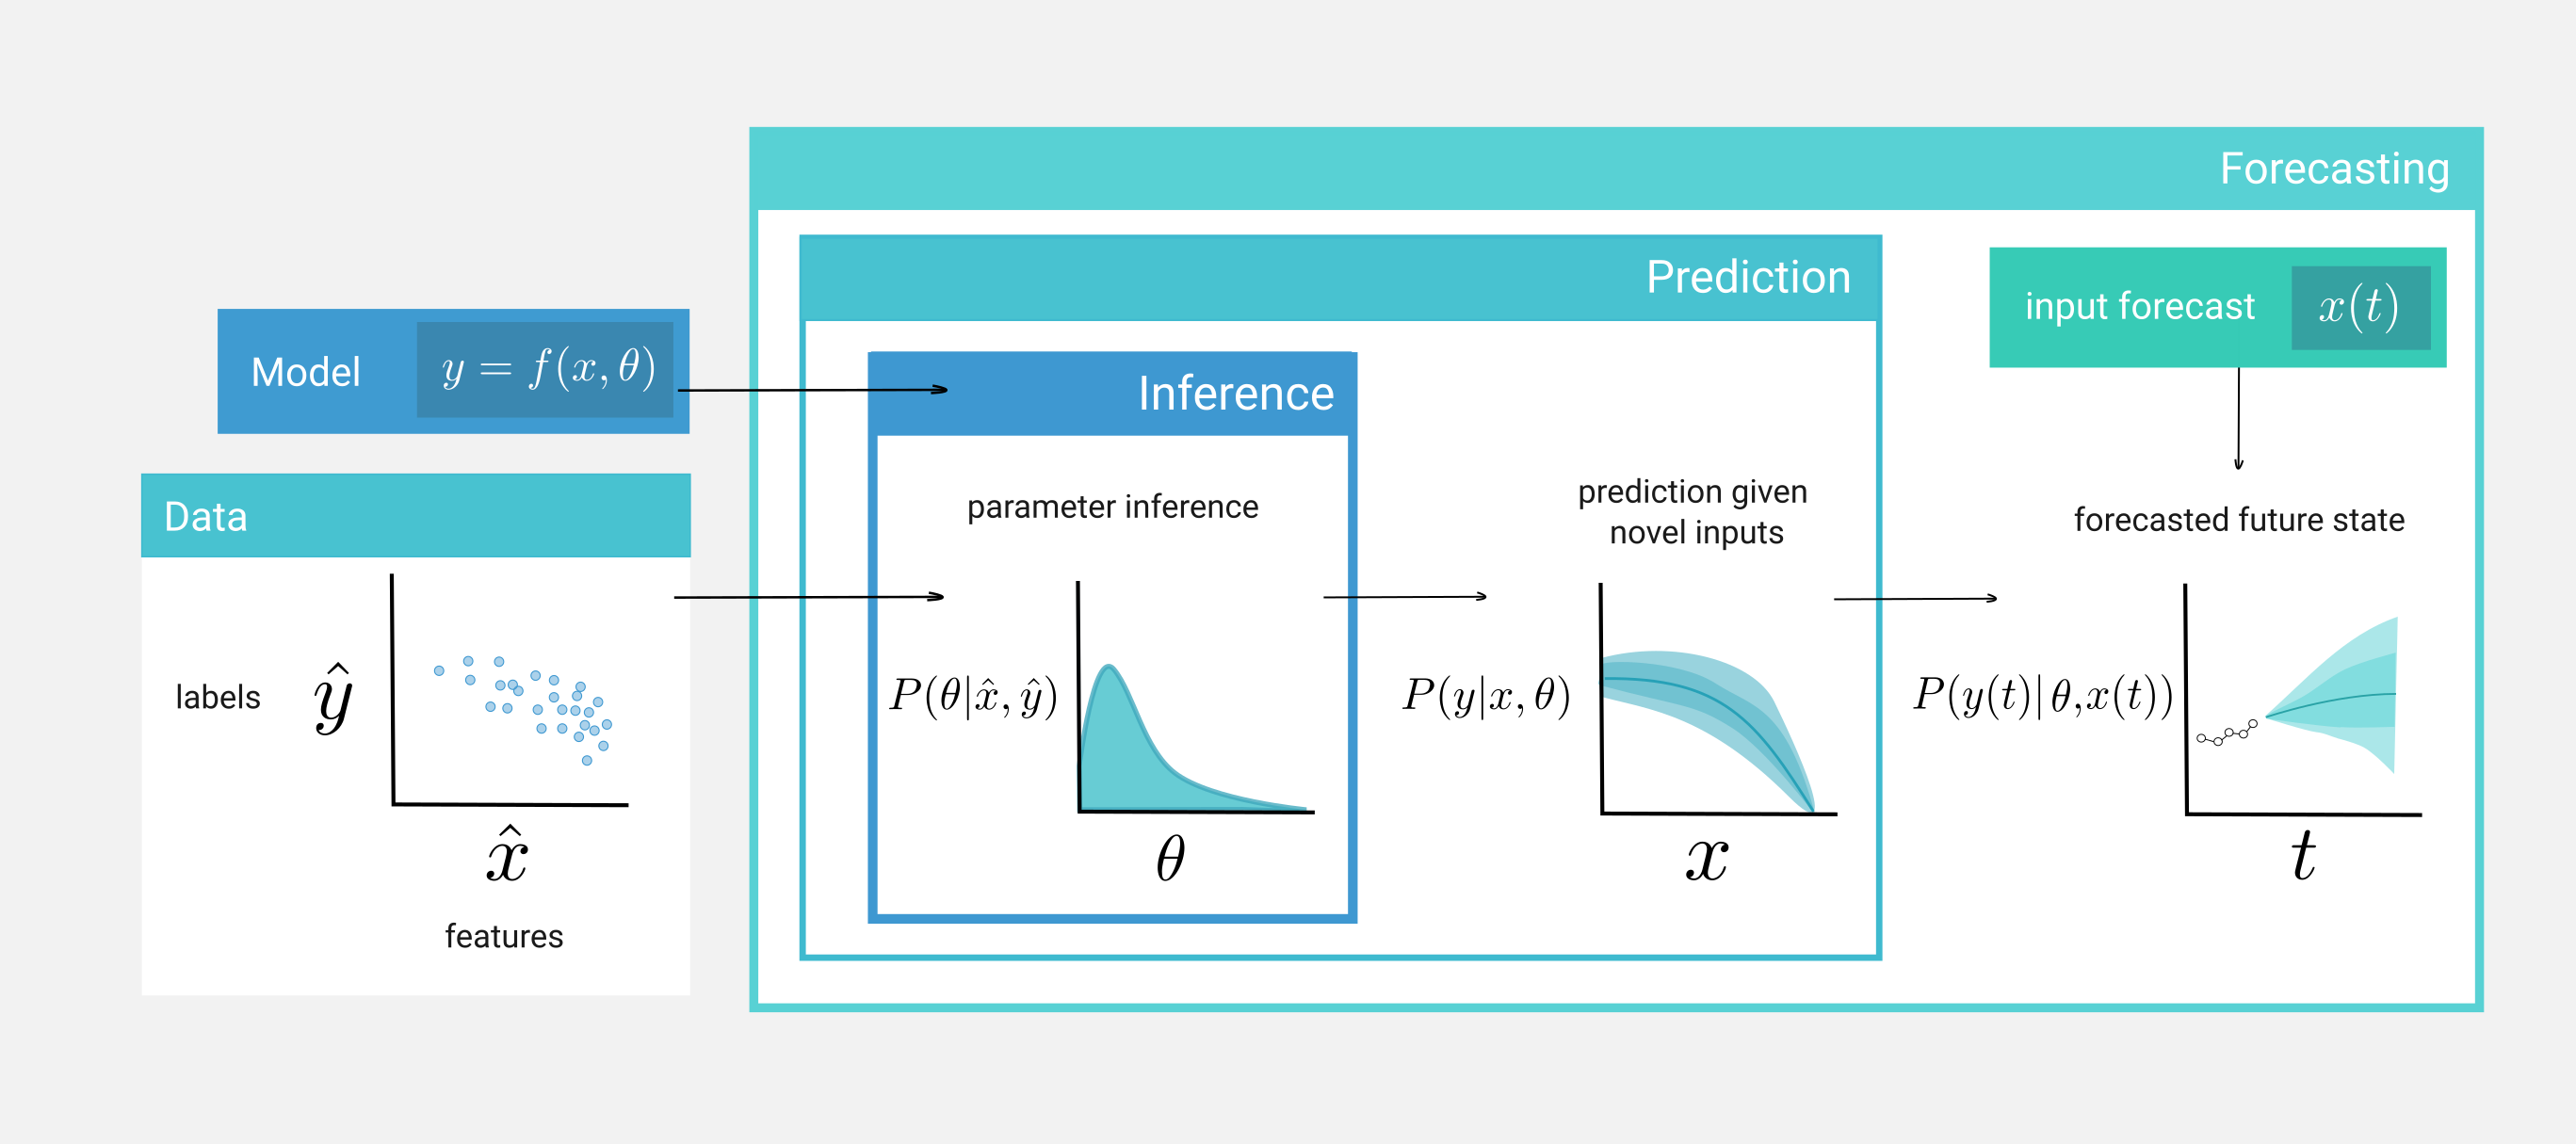
\includegraphics{figures/forecasting_v3.png}
\caption{The nested nature of developing predictive and forecasting
models, showcases the \emph{forward problem} and how this relies on a
hierarchical structure of the modelling process.}\label{fig:models}
}
\end{figure}

\hypertarget{what-do-you-need-to-build-a-predictive-model}{%
\subsubsection{What do you need to build a predictive
model?}\label{what-do-you-need-to-build-a-predictive-model}}

In order to build a predictive machine-learning model, one needs the
following: first, \textbf{data}, split into features \(\hat{x}\) and
labels \(\hat{y}\) (Box Figure Label). Second, a \textbf{model} \(f\),
which maps features \(x\) to labels \(y\) as a function of parameters
\(\theta\), i.e.~\(y = f(x, \theta)\). Third, a loss function
\(L(\hat{y}, y)\), which describes how far a model's prediction \(y\) is
from an empirical estimate \(\hat{y}\). Lastly, \textbf{priors} on
parameters, \(P(\theta)\). Another important step before fitting a model
is feature engineering: adjusting and reworking the predictors to better
uncover predictor-response relationships (Kuhn and Johnson 2019). This
can include projecting the predictors into a lower dimensional space, as
in our proof-of-concept.

\hypertarget{how-do-we-validate-a-predictive-model}{%
\subsubsection{How do we validate a predictive
model?}\label{how-do-we-validate-a-predictive-model}}

After model fitting, we inevitably want to see how ``good'' it is. One
of the context for validation is \emph{model comparison}, where we aim
to see which of a competing set of models provides the best explanation
for a data set. A naive initial approach is to simply compute the
average error between the model's prediction and the true data we have,
and choose the model with the smallest error---however this approach
inevitably results in \emph{overfitting}. One approach to avoid
overfitting is using information criteria (\emph{e.g.} AIC, BIC, MDL)
based around the heuristic that good models maximize the ratio of
information provided by the model to the number of parameters it has.
However, when the intended use-case of a model is prediction the
relevant form of validation is \emph{predictive accuracy}, which should
be tested with \emph{crossvalidation}. Crossvalidation methods divide
the original dataset into two---one which is used to fit the model
(called the \emph{training} set) and one used to validate its predictive
accuracy on the data that is hasn't ``seen'' yet (called the \emph{test}
set) (Bishop 2006). This procedure is often repeated for different
subdivisions of the dataset (Arlot and Celisse 2010).

\hypertarget{networks-and-interactions}{%
\subsection{Networks and Interactions}\label{networks-and-interactions}}

\hypertarget{why-predict-networks-and-interactions-at-the-same-time}{%
\subsubsection{Why predict networks and interactions at the same
time?}\label{why-predict-networks-and-interactions-at-the-same-time}}

Ecological networks are quite sparse (MacDonald, Banville, and Poisot
2020)---composed of a set of interactions, but also a larger set of
non-interactions. If we aim to predict the structure of networks from
the ``bottom-up''--- by considering each pairwise combination of \(S\)
different species---we are left with \(S^2\) interaction values to
estimate. Instead, we can use our existing understanding of the
mechanisms that structure ecological networks to whittle down the set of
feasible adjacency matrices, thereby reducing the amount of information
we must predict, and making the problem of predicting interactions less
daunting. The processes that structure ecological networks do not only
occur at the scale of interactions---there are also processes at the
network level which limit what interactions are possible. The realized
structure of a network is the synthesis of the interactions forming the
basis for network structure, and the network structure refining the
possible interactions---``Part makes whole, and whole makes part''
(Levins and Lewontin 1987).

\hypertarget{what-network-properties-should-we-should-use-to-inform-our-predictions-of-interactions}{%
\subsubsection{What network properties should we should use to inform
our predictions of
interactions?}\label{what-network-properties-should-we-should-use-to-inform-our-predictions-of-interactions}}

There are many dimensions of network structure (Delmas et al. 2018).
This might make the task of network structure prediction look daunting,
as the number of properties one could predict is immense. Yet there are
two reasons to begin with a single property, connectance (the ratio of
actual edges to possible edges in the network). First, connectance is
ecologically informative---it relates to resilience to invasion (Baiser,
Russell, and Lockwood 2010; Smith-Ramesh, Moore, and Schmitz 2016), can
increase robustness to extinction in food webs (Jennifer A. Dunne,
Williams, and Martinez 2002), while decreasing it in mutualistic
networks (Vieira and Almeida-Neto 2015), and connectance relates to
network stability (Landi et al. 2018). Second, most (if not all) network
properties co-vary with connectance (Poisot and Gravel 2014; Jennifer A.
Dunne, Williams, and Martinez 2002). We have models to estimate species
richness over space (Jenkins, Pimm, and Joppa 2013), and because we can
predict connectance from species richness, (MacDonald, Banville, and
Poisot 2020), we can then derive distributions of network properties
from estimates of richness alone. Therefore we suggest that predicting
the value of network connectance across space (and eventually time) is
most likely to be the most practical to formulate at the moment.

\hypertarget{how-do-we-predict-how-species-that-have-never-co-occurred-will-interact}{%
\subsubsection{How do we predict how species that have never co-occurred
will
interact?}\label{how-do-we-predict-how-species-that-have-never-co-occurred-will-interact}}

The probability of an interaction occurring depends on the likelihood of
co-occurrence in space and time (Poisot, Stouffer, and Gravel 2015;
Pichler et al. 2020). Given two species co-occur, a neutral approach to
probabilistic interactions would assume that the effect of abundances
and trait matching would have no effect (E. Canard et al. 2012).
However, functional-trait based proxies could enable better predictions
of ecological interactions. Selection on functional traits could cause
interactions to be conserved at some evolutionary scales, and therefore
predictions of interaction could be informed by phylogenetic analyses.
(Elmasri et al. 2020; Gómez, Verdú, and Perfectti 2010). Phylogenetic
matching in bipartite networks is consistent across scales (Poisot and
Stouffer 2018), even absent strong selective pressure (Coelho,
Rodrigues, and Rangel 2017).

A separate family of methods are based on network embedding (as in the
proof-of-concept). A network embedding projects each node of the network
into a lower-dimensional latent space. This enables us to represent the
structure of a network, which previously required the \(S^2\) dimensions
of an adjacency matrix, with a smaller number of dimensions. The
position of each node in this lower dimensional space is then treated as
a latent measurement corresponding to the role of that species in the
network (Becker et al. 2020). Species close together in the latent space
should interact with similar set of species (Rossberg et al. 2006; Rohr
et al. 2010). However, these models are sensitive to sampling biases as
they are limited to species for which there is already interaction data
(Becker et al. 2020).

\hypertarget{what-is-an-interaction-really}{%
\subsubsection{What is an interaction,
really?}\label{what-is-an-interaction-really}}

Interactions between species can be conceptualized in a multitude of
ways (mutualistic vs.~antagonistic, strong vs.~weak, symmetric
vs.~asymmetric, direct vs.~indirect) (Jordano 2016a; Morales-Castilla et
al. 2015). What is common to all definitions of interaction is that
\emph{at least} one of the species is affected by the presence of
another, either positively or negatively (Morales-Castilla et al. 2015).
Networks can be used to represent a variety of interaction types,
including: \emph{unipartite networks,} where each species can be linked
any other species, species (these are typically used to represent food
webs), \emph{bipartite networks} where there are two pools of species,
and all interactions occur between species in each pool, are typically
used for pairwise interactions (e.g.~hosts and parasites), and
\emph{k-partite networks:,} which serve as a way to expand to more than
two discrete sets of interacting species (e.g.~parasitoid webs, seed
dispersal networks, and pollination networks) (Pocock, Evans, and
Memmott 2012).

\hypertarget{what-about-interaction-strength}{%
\subsubsection{\texorpdfstring{What about interaction
\emph{strength}?}{What about interaction strength?}}\label{what-about-interaction-strength}}

Species interaction networks can also be used as means to quantify and
understand \emph{interaction strength}. Interaction strength, unlike the
qualitative presence or absence an interaction, is a continuous
measurement which attempts to quantify the effect of one species on
another. Interaction strength can generally be divided into two main
categories (as suggested by Berlow et al. (2004)): either the strength
of an interaction between individuals of each species, or the effect
that changes in one species population has on the dynamics of the other
species. Further, it can be measured either as the direct effect of one
species on another over a period of time (often in the units of biomass)
or the relative importance of one species on another (Heleno et al.
2014; Berlow et al. 2004; Wootton and Emmerson 2005). One recurring
observation throughout studies of interaction strengths is that networks
are often composed of many weak links and few strong links (Berlow et
al. 2004). The distribution of interaction strength within a network
informs on its stability (Neutel 2002; Ruiter, Neutel, and Moore 1995),
influences on the ecosystem functioning (Duffy 2002; Montoya, Rodríguez,
and Hawkins 2003) and our potential to improve multispecies models
(Wootton and Emmerson 2005). Seeing interaction strength within a
network as energy fluxes could also possibly lead to its integration
within the Biodiversity-Ecosystem Functioning (BEF) framework, which
could in return further improve even our understanding of community
dynamics and ecosystem functioning (Barnes et al. 2018a).

\hypertarget{how-are-interaction-strengths-actually-estimated}{%
\subsubsection{How are interaction strengths actually
estimated?}\label{how-are-interaction-strengths-actually-estimated}}

Before we attempt to make inferences from data, we must adapt a
conceptual framework to model interaction strength. One such framework
is functional foraging (Portalier et al. 2019), where the primary basis
for inferring interaction is based on an organism's traits, the
environment, and foraging behavior like searching, capture and handling
times. A different conceptual alternative, applicable in food-webs, is
metabolic based models, where body mass, metabolic demands, and energy
loss are used to infer energetic energy fluxes between organisms (Yodzis
and Innes 1992; Berlow et al. 2009). Energy can be seen as the common
currency that links every level of biology from individual organisms to
the whole ecosystem (Brown et al. 2004; Barnes et al. 2018b). A
(metabolically) bottom-up approach first estimates basal species
biomasses and compute the higher trophic-level species biomasses and
energetic demands from there (Berlow et al. 2009). Alternatively, a
metabolically top-down approach computes energy fluxes starting from the
top consumer downward toward producers (Barnes et al. 2018a). Food-web
energetics models can be incorporated at various resolutions for a
specific network, ranging from individual-based data to more lumped data
at the species level or trophic group, depending on data availability
(Barnes et al. 2018a).

\hypertarget{what-about-indirect-and-higher-order-interactions}{%
\subsubsection{What about indirect and higher-order
interactions?}\label{what-about-indirect-and-higher-order-interactions}}

Although network ecology often assumes that interactions go strictly
from one node to the other, the web of life is made up of a variety of
interactions. Indirect interactions---either higher-order interactions
between species, or interaction strengths that themselves interact ---
has gained interest in recent years (Golubski et al. 2016; Golubski and
Abrams 2011). One mathematical tool to describe these situations is
hypergraphs: hypergraphs are the generalization of a graph, allowing a
broad yet manageable approach to complex interactions (Carletti,
Fanelli, and Nicoletti 2020), allowing for particular interactions to
occur beyond a pair of nodes. An additional degree of complexity is
introduced by multi-layer networks (Hutchinson et al. 2019). Multi-layer
networks include edges across ``variants'' of the networks (timepoints,
locations, or environments). These can be particularly useful to account
for the metacommunity structure (Gross et al. 2020), or to understand
how dispersal can inform conservation action (Albert et al. 2017).
Ecological networks are intrinsically multi-layered (Pilosof et al.
2017). \emph{Prima facie}, increasing the dimensionality of the object
we need to predict (the multiple layers rather than a single network)
may make the problem complicated. But multi-layer networks encode
ecological constraints -- of dispersal, of evolution, and of niche
suitability. It is worth investigating if the multi-layer structure of
ecological networks could improve the predictibility of interactions, as
in social networks (Jalili et al. 2017; Najari et al. 2019; Yasami and
Safaei 2018).

\hypertarget{how-do-we-determine-what-interaction-networks-are-feasible}{%
\subsubsection{How do we determine what interaction networks are
feasible?}\label{how-do-we-determine-what-interaction-networks-are-feasible}}

For several decades, ecologists have aimed to understand how networks of
many interacting species persist through time. The diversity-stability
paradox, first explored by May (1974), shows that under a neutral set of
assumptions, ecological networks should become decreasingly stable as
the number of species increases. However, in the natural world we
observe networks of interactions that consist of far more species than
May's model predicts (Albouy et al. 2019). As a result, understanding
what aspects of the neutral assumptions of May's model are incorrect has
branched many investigations into the relationship between ecological
network structure and persistence (Allesina and Tang 2012). These
assumptions can be split into dynamical assumptions and topological
assumptions.

Topologically, we know that ecological networks are not structured
randomly. Some properties, like the aforementioned connectance, are
highly predictable (MacDonald, Banville, and Poisot 2020). Various
generative models of food-webs have been shown to fit empirical networks
more effectively than random models. These typically rely on network
embeddings, where each node (species) in the network is assigned a value
in a latent space, and the resulting network topology is generated
stochastically based on properties of the position of nodes in that
latent space. Generative network models have long used allometry as a
single-dimensional latent space---naturally we want to extend this to
traits in general (Allesina, Alonso, and Pascual 2008). The second
approach to understand stability is through \emph{dynamics}. Early
models of community dynamics rely on the assumption of linear
interaction effects. However, models of bioenergetic community dynamics
have shown promise in basing our understanding of dynamics in food-webs,
where the functional response of one species on another is grounded in
the understood relationship between allometry and metabolism (Delmas et
al. 2017). An additional consideration is the multidimensional nature of
``stability'' and ``feasibility'' (e.g resilience to environmental
change vs extinctions) (Domínguez-García, Dakos, and Kéfi 2019) and how
different disturbances propagate across levels of biological
organization (Kéfi et al. 2019; Gravel, Massol, and Leibold 2016).

\hypertarget{space}{%
\subsection{Space}\label{space}}

Although networks were initially used to describe the interactions
\emph{within} a community, interest in the last decade has shifted
towards understanding their structure and variation over space
(Trøjelsgaard and Olesen 2016; Baiser et al. 2019), and has established
network ecology as an important emerging component of biogeography and
macroecology.

\hypertarget{how-much-do-networks-vary-over-space}{%
\subsubsection{How much do networks vary over
space?}\label{how-much-do-networks-vary-over-space}}

Networks can vary across space either in their structural properties
(e.g. connectance or degree distribution) or in their composition
(identity of nodes and edges). Interestingly, variation in the
structural properties of ecological networks primarily responds to
changes in the size of the network. The number of links in ecological
networks scales with the number of species (MacDonald, Banville, and
Poisot 2020; Brose et al. 2004), and connectance and size drive the rest
of the structural properties of ecological networks (Poisot and Gravel
2014; Jennifer A. Dunne, Williams, and Martinez 2002; Riede et al.
2010). Species turnover in space results in changes in the composition
of ecological networks. But, this is not the only reason network
composition varies (Poisot, Stouffer, and Gravel 2015). Intraspecific
variation can result in interaction turnovers without changes in species
composition (Bolnick et al. 2011). Similarly, changes in species
abundances can lead to variation in interaction strengths (E. F. Canard
et al. 2014; Vázquez et al. 2007). Variation in the abiotic environment
and indirect interactions (Golubski et al. 2016) could modify the
occurrence and strength of individual interactions. Despite this,
empirical networks tend to share a common backbone (Mora et al. 2018)
and functional composition (Dehling et al. 2020) across space.

\hypertarget{how-do-we-predict-what-the-species-pool-at-a-particular-location-is}{%
\subsubsection{How do we predict what the species pool at a particular
location
is?}\label{how-do-we-predict-what-the-species-pool-at-a-particular-location-is}}

As the species pool forms the basis for network structure, predicting
which species are present at a particular location is essential to
predict networks across space. Species distribution models (SDMs) are
increasingly ubiquitous in macroecology--- these models predict the
range of a species based on known occurrences and environmental
conditions, such as climate and land cover (Guisan and Thuiller 2005;
Elith et al. 2006). Including interactions or co-occurrences in SDMs
generally improves predictive performance (Wisz et al. 2013).Several
approaches exist to combine multiple SDMs: community assemblage at a
particular site can be predicted either by combining independent
single-species SDMs (stacked-SDMs, SSDMs) or by directly modelling the
entire species assemblage and multiple species at the same time (joint
SDMs, JSDMs) (Norberg et al. 2019). Building on the JSDM framework,
hierarchical modeling of species communities (Ovaskainen et al. 2017)
has the advantage of capturing processes that structure communities.
Spatially Explicit Species Assemblage Modeling (SESAM) constrains SDM
predictions using macro-ecological models (Guisan and Rahbek 2011) ---
for example, variation in species richness across space can constrain
assemblage predictions (D'Amen et al. 2015).

The next step is to constrain distribution predictions using network
properties. This would also build on previous calls to adopt a
probabilistic view: there have been calls for a probabilistic species
pool (Karger et al. 2016), and more importantly including interactions
through Bayesian networks and propagating conditional dependencies has
generated better range predictions (Staniczenko et al. 2017). Blanchet,
Cazelles, and Gravel (2020) argue that the probabilistic view avoids
confusion between interactions and co-occurrences, but that it requires
prior knowledge of interactions. This could potentially be solved
through our framework of predicting networks first, interactions next,
and finally the realized species pool.

\hypertarget{how-do-we-combine-spatial-and-network-predictions}{%
\subsubsection{How do we combine spatial and network
predictions?}\label{how-do-we-combine-spatial-and-network-predictions}}

In order to predict networks across space, we need to combine multiple
models---one which predicts what the species pool will be at a given
location, and one to predict what interaction networks composed from
this species pool are likely (see fig.~\ref{fig:conceptual}). Both of
these models contain uncertainty, and when we combine them our
uncertainty from each to propagate into the combined model. The Bayesian
paradigm provides a convenient solution to this---if we have a chain of
models where each model feeds into the next, we can sample from the
posterior of the input models. A different approach is \emph{ensemble
modeling} which combines the predictions made be several models, where
each model is predicting the same thing (Parker 2013). Error
propagation, an important step in building any ecological model,
describes the effect of the uncertainty of input variables on the
uncertainty of output variables (Draper 1995; Parysow, Gertner, and
Westervelt 2000). Benke et al. (2018) identifies two broad approaches to
model error propagation: analytically using differential equations or
stochastically using Monte-Carlo simulation methods. Errors induced by
the spatial or temporal extrapolation of data also need to be taken into
account when estimating the uncertainty of a model's output (Peters and
Herrick 2004).

\hypertarget{what-is-the-spatial-scale-suitable-for-the-prediction-of-species-interactions}{%
\subsubsection{What is the spatial scale suitable for the prediction of
species
interactions?}\label{what-is-the-spatial-scale-suitable-for-the-prediction-of-species-interactions}}

As described above, we can use different trait-based proxies to predict
potential interactions. The choice of such proxies should be
theoretically linked to the spatial scale we are using in our prediction
(Wiens 1989). At some scales we can use morphological traits of
co-occurring species to assess the probability of interaction between
them (Bartomeus et al. 2016). This translates to a spatial extent that
does not necessarily capture the entire distribution of a given set of
species, with a resolution that is sufficient to capture the
phenotypical variability of the species. At some scales, we can infer
interactions through the phylogenetic similarity between species,
assuming their functional traits are themselves are conserved (Gómez,
Verdú, and Perfectti 2010). On evolutionary scales where the niche is
conserved, we can think of the probability that one species will
interact with another as the distance between them in niche-space
(Desjardins-Proulx et al. 2017). At the smallest scales, we may be
interested in predicting behavioral traits like foraging behavior
(Bartomeus et al. 2016). At this point, the spatial resolution in this
case should is fine enough that a model may be precise in a given
system, but much less generalizable. At this scale it is also important
to consider abundance's effect on probability of an encounter (Wells and
O'Hara 2013).

\hypertarget{time}{%
\subsection{Time}\label{time}}

\hypertarget{why-should-we-forecast-species-interaction-networks}{%
\subsubsection{Why should we forecast species interaction
networks?}\label{why-should-we-forecast-species-interaction-networks}}

Forecasting species interactions are critical for informing ecosystem
management (Harvey et al. 2017) and systematic conservation
prioritization (Pollock et al. 2020), and for anticipating extinctions
and their consequences (McDonald-Madden et al. 2016; McWilliams et al.
2019). Ecological interactions shape species distributions at both local
and broad spatial scales, and including interactions in SDM models
typically improves predictive performance (M. B. Araújo and Luoto 2007;
Wisz et al. 2013; Pigot and Tobias 2013). However, these tend to rely on
approaches involving estimating pairwise dependencies based on
cooccurance, using surrogates for biotic-interaction gradients, and
hybridizing SDMs with dynamic models (Wisz et al. 2013). Most existing
models to predict the future distribution of species ignore interactions
(Urban et al. 2016). Changes in species ranges and phenology will
inevitably create spatiotemporal mismatches and affect encounter rates
between species (Gilman et al. 2010), which will further shift the
distribution of species across space. New interactions will also appear
between species that are not currently co-occuring (Gilman et al. 2010).
Only by forecasting how species will interact can we hope to have an
accurate portrait of how biodiversity will be distributed under the
future climate.

Forecasting how climate change will alter biodiversity is also crucial
for maximizing conservation outcomes. Improving SDMs through
interactions is crucial for conservation, as nearly 30\% of models in
SDM studies are used to assess population declines or landscape ability
to support populations (M. B. Araújo et al. 2019). Reliable predictions
about how ecological networks will change over time will give us
critical information that could be communicated to decision-makers and
the scientific community about what are future environmental risks
awaiting and how to mitigate them (Kindsvater et al. 2018). Not only
this, but how biodiversity is structured influence the functioning of
the whole ecosystem, community stability and persistence Stouffer and
Bascompte (2010). Will climate change impact the distribution of network
properties (e.g.~connectance)? If so, which regions or species groups
need special conservation efforts? These overarching questions are yet
to be answered (but see Albouy et al. 2013; Kortsch et al. 2015; Hattab
et al. 2016). We believe that the path toward forecasting ecological
networks provides useful guidelines to ultimately better predict how
climate change will affect the different dimensions of biodiversity and
ecosystem functioning.

\hypertarget{how-do-we-turn-a-predictive-model-into-a-forecasting-model}{%
\subsubsection{How do we turn a predictive model into a forecasting
model?}\label{how-do-we-turn-a-predictive-model-into-a-forecasting-model}}

On some scales, empirical time-series encode enough information about
ecological processes for machine-learning approaches to make accurate
forecasts. However, there is an intrinsic limit to the predictability of
ecological time-series (Pennekamp et al. 2019). A forecast inherently
has a \emph{resolution limit} in space, time, and organization. For
example, one could never hope to predict the precise abundance of every
species on Earth on every day hundreds of years into the future. There
is often a trade-off between the resolution and horizon of forecast,
\emph{e.g.}, a lower resolution forecast, like primary production will
be at a maximum in the summer, is likely to be true much further into
the future than a higher resolution forecast. If we want to forecast the
structure of ecological networks beyond the forecasting horizon of
time-series based methods, we need forecasts of our predictive model's
inputs--- a forecast of the distribution of both environmental
conditions and the potential species pool across space
(fig.~\ref{fig:models}).

\hypertarget{how-can-we-validate-a-forecasting-model}{%
\subsubsection{How can we validate a forecasting
model?}\label{how-can-we-validate-a-forecasting-model}}

Often the purpose of building a forecasting model to inform
\emph{present} action (Dietze et al. 2018). Yet, the nature of
forecasting---trying to predict the future---is that you can only know
if a forecast is ``right'' once it is too late to change it. If we want
to maximize the chance that reality falls within a forecasting model's
predictions, there are two directions to approach this problem: the
first is to extend model validation techniques to a forecasting context,
and the second is to attempt to maximize the amount of uncertainty in
the forecast without compromising its resolution. Crossvalidation (see
\emph{How do we validate a predictive model?}) can be used to test the
efficacy of a forecasting model. Given a time-series of \(N\)
observations, a model can iteratively be trained on the first \(n\)
time-points of data, and the forecasting model's accuracy can be
evaluated on the remaining time-points it hasn't ``seen'' (Bishop 2006).
This enables us to understand both how much temporal data is required
for a model to be robust, and also enables us to explore the
\emph{forecasting horizon} of a process. Further, this approach can also
be applied in the opposite temporal direction--- if we have reliable
data from the past, ``hindcasting'' can also be used to test a
forecast's robustness.

However, these methods inevitably bump into a hard-limitation on what is
feasible for a forecasting model. The future is uncertain. Any empirical
time-series we use to validate a model was collected in past conditions
that may not persist into the future. Any system we wish to forecast
will undergo only one of many possible scenarios, yet we can only
observe the realized outcome of the system under the scenario that
actually unfolds. It is therefore impossible to assess the quality of a
forecasting model in scenarios that remain hypothetical. If the goal is
to maximize the probability that reality will fall within the forecast's
estimates, forecasts should incorporate as much uncertainty about the
future scenario as possible---one way to do this is ensemble modeling
(Parker 2013). However, as we increase the amount of uncertainty we
incorporate into a forecasting model, the resolution of the forecast's
predictions could shrink (Lei and Whitaker 2017), and therefore the
modeler be mindful of the trade-off between resolution and accuracy
where developing any forecast.

\hypertarget{conclusion-why-should-we-predict-species-interaction-networks}{%
\section{Conclusion: why should we predict species interaction
networks?}\label{conclusion-why-should-we-predict-species-interaction-networks}}

Because we almost can, and because we definitely should. A better
understanding of species interactions, and the networks they form, would
help unify the fields of community, network, and spatial ecology;
improve the quantification of the functional relationships between
species (Dehling and Stouffer 2018; O'Connor et al. 2020); re-evaluate
metacommunities in light of network structure (Guzman et al. 2019); and
enable a new line of research into the biogeography of species
interactions (Massol et al. 2017; Braga et al. 2019) which incorporates
a synthesis of both Eltonian and Grinnellian niche (Gravel et al. 2019).
Further, the ability to reliably predict and forecast species
interactions would inform conservation efforts for protecting species,
communities, and ecosystems. Integration of species interactions into
the assessment of vulnerability to climate change is a needed
methodological advance (Foden and Young 2016). International panels draw
on models to establish scientific consensus (M. B. Araújo et al. 2019),
and they can be improved through more effective prediction of species
distributions and interactions (Syfert et al. 2014). Further, recent
studies argue for a shift in focus from species to interaction networks
for biodiversity conservation to better ecosystem processes (Harvey et
al. 2017).

We should invest in network prediction because the right conditions to
do so reliably and rapidly, including forecasting, are beginning to
emerge. Given the possible benefits to a variety of ecological
disciplines that would result from an increased ability to predict
ecological networks and their structure, we feel strongly that the
research agenda we outline here should be picked up by the community.
Although novel technologies are bringing massive amounts of data to some
parts of ecology (primarily environmental DNA and remote sensing, but
now more commonly image analysis and bioacoustics), it is even more
important to be intentional about \emph{reconciling} data. This involves
not only the scholarly work of understand the processes that the data
encode, and whether they speak to scales that are compatible, but also
the groundwork of developing pipelines to bridge the ever-expanding gap
between ``high-throughput'' and ``low-throughput'' sampling methods. An
overall increase in the volume of data will not result in an increase of
our predictive capacity as long as this data increase is limited to
specific aspects of the problem. In the areas we highlight in
fig.~\ref{fig:conceptual}, many data steps are still limiting:
documenting empirical interactions is natural history work that doesn't
lend itself to systematic automation; expert knowledge is by design a
social process that may be slightly accelerated by text mining and
natural language processing (but is not yet, or not routinely or at
scale). These limitations are affecting our ability to reconstruct
networks.

But the tools to which we feed these data, incomplete as they may be,
are gradually getting better; that is, they can do predictions faster,
they handle uncertainty and propagate it well, and they can accomodate
data volumes than are lower than we may expect (Pichler et al. 2020). It
is clear attempting to predict the structure of ecological networks at
any scale is a methodological and ecological challenge; yet it will
result in qualitative changes in our understanding of complex adaptive
systems, as well as changes to our ability to leverage information about
network structure for conservation decision. It is perhaps even more
important to forecast the structure of ecological networks because it is
commonly neglected as a facet of biodiversity that can (and should) be
managed. In fact, none of the Aichi targets mention biostructure or its
protection, despite this being recognized as an important task (McCann
2007), either implicitely or explicitely. Being able to generate
reliable datasets on networks in space or time will make this
information more actionable.

\textbf{Acknowledgements:} TS, NF, TP are funded by a donation from the
Courtois Foundation; FB, NF, and TP are funded by IVADO; BM is funded by
the NSERC Alexander Graham Bell Canada Graduate Scholarship and the
FRQNT master's scholarship; FB, GD, NF, and GH are funded by the NSERC
BIOS² CREATE program; DC, TS, LP, and TP are funded by the Canadian
Institute of Ecology \& Evolution; this research was enabled in part by
support provided by Calcul Québec (www.calculquebec.ca) and Compute
Canada (www.computecanada.ca).

\hypertarget{references}{%
\section*{References}\label{references}}
\addcontentsline{toc}{section}{References}

\hypertarget{refs}{}
\begin{CSLReferences}{1}{0}
\leavevmode\hypertarget{ref-deAguiar2019RevBia}{}%
Aguiar, Marcus A. M. de, Erica A. Newman, Mathias M. Pires, Justin D.
Yeakel, Carl Boettiger, Laura A. Burkle, Dominique Gravel, et al. 2019.
{``Revealing Biases in the Sampling of Ecological Interaction
Networks.''} \emph{PeerJ} 7 (September): e7566.
\url{https://doi.org/10.7717/peerj.7566}.

\leavevmode\hypertarget{ref-Albert2017AppNet}{}%
Albert, Cécile H., Bronwyn Rayfield, Maria Dumitru, and Andrew Gonzalez.
2017. {``Applying Network Theory to Prioritize Multispecies Habitat
Networks That Are Robust to Climate and Land-Use Change: Prioritizing a
Network for Biodiversity.''} \emph{Conservation Biology} 31 (6):
1383--96. \url{https://doi.org/10.1111/cobi.12943}.

\leavevmode\hypertarget{ref-Albouy2019MarFis}{}%
Albouy, Camille, Philippe Archambault, Ward Appeltans, Miguel B. Araújo,
David Beauchesne, Kevin Cazelles, Alyssa R. Cirtwill, et al. 2019.
{``The Marine Fish Food Web Is Globally Connected.''} \emph{Nature
Ecology \& Evolution} 3 (8): 1153--61.
\url{https://doi.org/10.1038/s41559-019-0950-y}.

\leavevmode\hypertarget{ref-Albouy2013ProCli}{}%
Albouy, Camille, François Guilhaumon, Fabien Leprieur, Frida Ben Rais
Lasram, Samuel Somot, Roland Aznar, Laure Velez, François Le Loc'h, and
David Mouillot. 2013. {``Projected Climate Change and the Changing
Biogeography of Coastal Mediterranean Fishes.''} Edited by Peter
Pearman. \emph{Journal of Biogeography} 40 (3): 534--47.
\url{https://doi.org/10.1111/jbi.12013}.

\leavevmode\hypertarget{ref-Albrecht2018PlaAni}{}%
Albrecht, Jörg, Alice Classen, Maximilian G. R. Vollstädt, Antonia Mayr,
Neduvoto P. Mollel, David Schellenberger Costa, Hamadi I. Dulle, et al.
2018. {``Plant and Animal Functional Diversity Drive Mutualistic Network
Assembly Across an Elevational Gradient.''} \emph{Nature Communications}
9 (1): 3177. \url{https://doi.org/10.1038/s41467-018-05610-w}.

\leavevmode\hypertarget{ref-Allesina2008GenMod}{}%
Allesina, Stefano, David Alonso, and Mercedes Pascual. 2008. {``A
General Model for Food Web Structure.''} \emph{Science} 320 (5876):
658--61. \url{https://doi.org/10.1126/science.1156269}.

\leavevmode\hypertarget{ref-Allesina2012StaCri}{}%
Allesina, Stefano, and Si Tang. 2012. {``Stability Criteria for Complex
Ecosystems.''} \emph{Nature} 483 (7388): 205--8.
\url{https://doi.org/10.1038/nature10832}.

\leavevmode\hypertarget{ref-Antoniou2018DatAug}{}%
Antoniou, Antreas, Amos Storkey, and Harrison Edwards. 2018. {``Data
Augmentation Generative Adversarial Networks.''} \emph{arXiv:1711.04340
{[}cs, Stat{]}}, March. \url{http://arxiv.org/abs/1711.04340}.

\leavevmode\hypertarget{ref-Araujo2008NetAna}{}%
Araújo, Márcio S., Paulo R. Guimarães, Richard Svanbäck, Aluisio
Pinheiro, Paulo Guimarães, Sérgio F. dos Reis, and Daniel I. Bolnick.
2008. {``Network Analysis Reveals Contrasting Effects of Intraspecific
Competition on Individual Vs. Population Diets.''} \emph{Ecology} 89
(7): 1981--93. \url{https://doi.org/10.1890/07-0630.1}.

\leavevmode\hypertarget{ref-Araujo2019StaDis}{}%
Araújo, Miguel B., Robert P. Anderson, A. Márcia Barbosa, Colin M.
Beale, Carsten F. Dormann, Regan Early, Raquel A. Garcia, et al. 2019.
{``Standards for Distribution Models in Biodiversity Assessments.''}
\emph{Science Advances} 5 (1): eaat4858.
\url{https://doi.org/10.1126/sciadv.aat4858}.

\leavevmode\hypertarget{ref-Araujo2007ImpBio}{}%
Araújo, Miguel B., and Miska Luoto. 2007. {``The Importance of Biotic
Interactions for Modelling Species Distributions Under Climate
Change.''} \emph{Global Ecology and Biogeography} 16 (6): 743--53.
\url{https://doi.org/10.1111/j.1466-8238.2007.00359.x}.

\leavevmode\hypertarget{ref-Arlot2010SurCro}{}%
Arlot, Sylvain, and Alain Celisse. 2010. {``A Survey of Cross-Validation
Procedures for Model Selection.''} \emph{Statistics Surveys} 4: 40--79.
\url{https://doi.org/10.1214/09-SS054}.

\leavevmode\hypertarget{ref-Baiser2019EcoRul}{}%
Baiser, Benjamin, Dominique Gravel, Alyssa R. Cirtwill, Jennifer A.
Dunne, Ashkaan K. Fahimipour, Luis J. Gilarranz, Joshua A. Grochow, et
al. 2019. {``Ecogeographical Rules and the Macroecology of Food Webs.''}
\emph{Global Ecology and Biogeography} 28 (9): 1204--18.
\url{https://doi.org/10.1111/geb.12925}.

\leavevmode\hypertarget{ref-Baiser2010ConDet}{}%
Baiser, Benjamin, Gareth J. Russell, and Julie L. Lockwood. 2010.
{``Connectance Determines Invasion Success via Trophic Interactions in
Model Food Webs.''} \emph{Oikos} 119 (12): 1970--76.
\url{https://doi.org/10.1111/j.1600-0706.2010.18557.x}.

\leavevmode\hypertarget{ref-Barnes2018EneFlu}{}%
Barnes, Andrew D., Malte Jochum, Jonathan S. Lefcheck, Nico Eisenhauer,
Christoph Scherber, Mary I. O'Connor, Peter de Ruiter, and Ulrich Brose.
2018a. {``Energy Flux: The Link Between Multitrophic Biodiversity and
Ecosystem Functioning.''} \emph{Trends in Ecology \& Evolution} 33 (3):
186--97. \url{https://doi.org/10.1016/j.tree.2017.12.007}.

\leavevmode\hypertarget{ref-Barnes2018EneFlua}{}%
---------. 2018b. {``Energy Flux: The Link Between Multitrophic
Biodiversity and Ecosystem Functioning.''} \emph{Trends in Ecology \&
Evolution} 33 (3): 186--97.
\url{https://doi.org/10.1016/j.tree.2017.12.007}.

\leavevmode\hypertarget{ref-Bartomeus2016ComFra}{}%
Bartomeus, Ignasi, Dominique Gravel, Jason M. Tylianakis, Marcelo A.
Aizen, Ian A. Dickie, and Maud Bernard-Verdier. 2016. {``A Common
Framework for Identifying Linkage Rules Across Different Types of
Interactions.''} \emph{Functional Ecology} 30 (12): 1894--1903.
\url{https://doi.org/10.1111/1365-2435.12666}.

\leavevmode\hypertarget{ref-Becker2020PreWil}{}%
Becker, Daniel J., Gregory F. Albery, Anna R. Sjodin, Timothée Poisot,
Tad A. Dallas, Evan A. Eskew, Maxwell J. Farrell, et al. 2020.
{``Predicting Wildlife Hosts of Betacoronaviruses for SARS-CoV-2
Sampling Prioritization: A Modeling Study.''} Preprint. Ecology.
\url{https://doi.org/10.1101/2020.05.22.111344}.

\leavevmode\hypertarget{ref-Benke2018ErrPro}{}%
Benke, K. K., S. Norng, N. J. Robinson, L. R. Benke, and T. J. Peterson.
2018. {``Error Propagation in Computer Models: Analytic Approaches,
Advantages, Disadvantages and Constraints.''} \emph{Stochastic
Environmental Research and Risk Assessment} 32 (10): 2971--85.
\url{https://doi.org/10.1007/s00477-018-1555-8}.

\leavevmode\hypertarget{ref-Bennett2019PotPit}{}%
Bennett, Alison E., Darren M. Evans, and Jeff R. Powell. 2019.
{``Potentials and Pitfalls in the Analysis of Bipartite Networks to
Understand Plantmicrobe Interactions in Changing Environments.''}
\emph{Functional Ecology} 33 (1): 107--17.
\url{https://doi.org/10.1111/1365-2435.13223}.

\leavevmode\hypertarget{ref-Berlow2009SimPre}{}%
Berlow, Eric L., Jennifer A. Dunne, Neo D. Martinez, Philip B. Stark,
Richard J. Williams, and Ulrich Brose. 2009. {``Simple Prediction of
Interaction Strengths in Complex Food Webs.''} \emph{Proceedings of the
National Academy of Sciences} 106 (1): 187--91.
\url{https://doi.org/10.1073/pnas.0806823106}.

\leavevmode\hypertarget{ref-Berlow2004IntStr}{}%
Berlow, Eric L., Anje-Margiet Neutel, Joel E. Cohen, Peter C. de Ruiter,
Bo Ebenman, Mark Emmerson, Jeremy W. Fox, et al. 2004. {``Interaction
Strengths in Food Webs: Issues and Opportunities.''} \emph{Journal of
Animal Ecology} 73 (3): 585--98.
\url{https://doi.org/10.1111/j.0021-8790.2004.00833.x}.

\leavevmode\hypertarget{ref-Bezanson2017JulFre}{}%
Bezanson, J., A. Edelman, S. Karpinski, and V. Shah. 2017. {``Julia: A
Fresh Approach to Numerical Computing.''} \emph{SIAM Review} 59 (1):
65--98. \url{https://doi.org/10.1137/141000671}.

\leavevmode\hypertarget{ref-Bishop2006PatRec}{}%
Bishop, Christopher M. 2006. \emph{Pattern Recognition and Machine
Learning}. Information Science and Statistics. New York: Springer.

\leavevmode\hypertarget{ref-Blanchet2020CooNot}{}%
Blanchet, F. Guillaume, Kevin Cazelles, and Dominique Gravel. 2020.
{``Co-Occurrence Is Not Evidence of Ecological Interactions.''}
\emph{Ecology Letters} 23 (7): 1050--63.
\url{https://doi.org/10.1111/ele.13525}.

\leavevmode\hypertarget{ref-Bohan2011AutDis}{}%
Bohan, David A., Geoffrey Caron-Lormier, Stephen Muggleton, Alan
Raybould, and Alireza Tamaddoni-Nezhad. 2011. {``Automated Discovery of
Food Webs from Ecological Data Using Logic-Based Machine Learning.''}
\emph{PLOS ONE} 6 (12): e29028.
\url{https://doi.org/10.1371/journal.pone.0029028}.

\leavevmode\hypertarget{ref-Bohan2017NexGlo}{}%
Bohan, David A., Corinne Vacher, Alireza Tamaddoni-Nezhad, Alan
Raybould, Alex J. Dumbrell, and Guy Woodward. 2017. {``Next-Generation
Global Biomonitoring: Large-Scale, Automated Reconstruction of
Ecological Networks.''} \emph{Trends in Ecology \& Evolution} 32 (7):
477--87. \url{https://doi.org/10.1016/j.tree.2017.03.001}.

\leavevmode\hypertarget{ref-Bolnick2011WhyInt}{}%
Bolnick, Daniel I., Priyanga Amarasekare, Márcio S. Araújo, Reinhard
Bürger, Jonathan M. Levine, Mark Novak, Volker H. W. Rudolf, Sebastian
J. Schreiber, Mark C. Urban, and David A. Vasseur. 2011. {``Why
Intraspecific Trait Variation Matters in Community Ecology.''}
\emph{Trends in Ecology \& Evolution} 26 (4): 183--92.
\url{https://doi.org/10.1016/j.tree.2011.01.009}.

\leavevmode\hypertarget{ref-Braga2019SpaAna}{}%
Braga, J, Laura J. Pollock, C. Barros, J. Montoya, Dominique Gravel,
Luigi Maiorano, Gentile Francesco Ficetola, Stéphane Dray, and Wilfried
Thuiller. 2019. {``Spatial Analyses of Multi-Trophic Terrestrial
Vertebrate Assemblages in Europe.''} \emph{Global Ecology and
Biogeography} 28 (11): 1636--48.

\leavevmode\hypertarget{ref-Brose2004UniSpa}{}%
Brose, Ulrich, Annette Ostling, Kateri Harrison, and Neo D. Martinez.
2004. {``Unified Spatial Scaling of Species and Their Trophic
Interactions.''} \emph{Nature} 428 (6979): 167--71.
\url{https://doi.org/10.1038/nature02297}.

\leavevmode\hypertarget{ref-Brown2004MetThe}{}%
Brown, James H., James F. Gillooly, Andrew P. Allen, Van M. Savage, and
Geoffrey B. West. 2004. {``Toward a Metabolic Theory of Ecology.''}
\emph{Ecology} 85 (7): 1771--89. \url{https://doi.org/10.1890/03-9000}.

\leavevmode\hypertarget{ref-Burkle2011FutPla}{}%
Burkle, L. A., and R. Alarcon. 2011. {``The Future of Plant-Pollinator
Diversity: Understanding Interaction Networks Across Time, Space, and
Global Change.''} \emph{American Journal of Botany} 98 (3): 528--38.
\url{https://doi.org/10.3732/ajb.1000391}.

\leavevmode\hypertarget{ref-Burkle2013PlaInt}{}%
Burkle, L. A., J. C. Marlin, and T. M. Knight. 2013. {``Plant-Pollinator
Interactions over 120 Years: Loss of Species, Co-Occurrence, and
Function.''} \emph{Science} 339 (6127): 1611--15.
\url{https://doi.org/10.1126/science.1232728}.

\leavevmode\hypertarget{ref-Canard2014EmpEva}{}%
Canard, E. F., N. Mouquet, D. Mouillot, M. Stanko, D. Miklisova, and D.
Gravel. 2014. {``Empirical Evaluation of Neutral Interactions in
Host-Parasite Networks.''} \emph{The American Naturalist} 183 (4):
468--79. \url{https://doi.org/10.1086/675363}.

\leavevmode\hypertarget{ref-Canard2012EmeStr}{}%
Canard, Elsa, Nicolas Mouquet, Lucile Marescot, Kevin J. Gaston,
Dominique Gravel, and David Mouillot. 2012. {``Emergence of Structural
Patterns in Neutral Trophic Networks.''} \emph{PLOS ONE} 7 (8): e38295.
\url{https://doi.org/10.1371/journal.pone.0038295}.

\leavevmode\hypertarget{ref-Carletti2020DynSys}{}%
Carletti, Timoteo, Duccio Fanelli, and Sara Nicoletti. 2020.
{``Dynamical Systems on Hypergraphs.''} \emph{Journal of Physics:
Complexity} 1 (3): 035006.
\url{https://doi.org/10.1088/2632-072X/aba8e1}.

\leavevmode\hypertarget{ref-Carpenter2002EcoFut}{}%
Carpenter, Stephen R. 2002. {``Ecological Futures: Building an Ecology
of the Long Now.''} \emph{Ecology} 83 (8): 2069--83.

\leavevmode\hypertarget{ref-Chawla2010DatMin}{}%
Chawla, Nitesh V. 2010. {``Data Mining for Imbalanced Datasets: An
Overview.''} In \emph{Data Mining and Knowledge Discovery Handbook},
edited by Oded Maimon and Lior Rokach, 875--86. Boston, MA: Springer US.
\url{https://doi.org/10.1007/978-0-387-09823-4_45}.

\leavevmode\hypertarget{ref-Christin2019AppDee}{}%
Christin, Sylvain, Éric Hervet, and Nicolas Lecomte. 2019.
{``Applications for Deep Learning in Ecology.''} \emph{Methods in
Ecology and Evolution} 10 (10): 1632--44.
\url{https://doi.org/10.1111/2041-210X.13256}.

\leavevmode\hypertarget{ref-Chuang2018AdvCon}{}%
Chuang, Kangway V., and Michael J. Keiser. 2018. {``Adversarial Controls
for Scientific Machine Learning.''} \emph{Acs Chemical Biology} 13 (10):
2819--21. \url{https://doi.org/10.1021/acschembio.8b00881}.

\leavevmode\hypertarget{ref-Coelho2017NeuBio}{}%
Coelho, Marco Túlio Pacheco, João Fabrício Mota Rodrigues, and Thiago F.
Rangel. 2017. {``Neutral Biogeography of Phylogenetically Structured
Interaction Networks.''} \emph{Ecography} 40 (12): 1467--74.
\url{https://doi.org/10.1111/ecog.02780}.

\leavevmode\hypertarget{ref-Creer2016EcoSF}{}%
Creer, Simon, Kristy Deiner, Serita Frey, Dorota Porazinska, Pierre
Taberlet, W. Kelley Thomas, Caitlin Potter, and Holly M. Bik. 2016.
{``The Ecologist's Field Guide to Sequence-Based Identification of
Biodiversity.''} \emph{Methods in Ecology and Evolution} 7 (9):
1008--18. \url{https://doi.org/10.1111/2041-210X.12574}.

\leavevmode\hypertarget{ref-Cutler2007RanFor}{}%
Cutler, D. Richard, Thomas C. Edwards, Karen H. Beard, Adele Cutler, and
Kyle T. Hess. 2007. {``Random Forests for Classification in Ecology.''}
\emph{Ecology} 88 (11): 2783--92.
\url{https://doi.org/10.1890/07-0539.1}.

\leavevmode\hypertarget{ref-DAmen2015UsiSpe}{}%
D'Amen, Manuela, Anne Dubuis, Rui F. Fernandes, Julien Pottier, Loïc
Pellissier, and Antoine Guisan. 2015. {``Using Species Richness and
Functional Traits Predictions to Constrain Assemblage Predictions from
Stacked Species Distribution Models.''} \emph{Journal of Biogeography}
42 (7): 1255--66. \url{https://doi.org/10.1111/jbi.12485}.

\leavevmode\hypertarget{ref-Dehling2020SimCom}{}%
Dehling, D. Matthias, Guadalupe Peralta, Irene M. A. Bender, Pedro G.
Blendinger, Katrin Böhning-Gaese, Marcia C. Muñoz, Eike Lena Neuschulz,
et al. 2020. {``Similar Composition of Functional Roles in Andean
Seed-Dispersal Networks, Despite High Species and Interaction
Turnover.''} \emph{Ecology} 101 (7).
\url{https://doi.org/10.1002/ecy.3028}.

\leavevmode\hypertarget{ref-Dehling2018BriElt}{}%
Dehling, D. Matthias, and Daniel B. Stouffer. 2018. {``Bringing the
Eltonian Niche into Functional Diversity.''} \emph{Oikos} 127 (12):
1711--23. \url{https://doi.org/10.1111/oik.05415}.

\leavevmode\hypertarget{ref-Delmas2018AnaEco}{}%
Delmas, Eva, Mathilde Besson, Marie-Hélène Brice, Laura A. Burkle,
Giulio V. Dalla Riva, Marie-Josée Fortin, Dominique Gravel, et al. 2018.
{``Analysing Ecological Networks of Species Interactions.''}
\emph{Biological Reviews}, June, 112540.
\url{https://doi.org/10.1111/brv.12433}.

\leavevmode\hypertarget{ref-Delmas2017SimBio}{}%
Delmas, Eva, Ulrich Brose, Dominique Gravel, Daniel B. Stouffer, and
Timothée Poisot. 2017. {``Simulations of Biomass Dynamics in Community
Food Webs.''} \emph{Methods in Ecology and Evolution} 8 (7): 881--86.
\url{https://doi.org/10.1111/2041-210X.12713}.

\leavevmode\hypertarget{ref-Desjardins-Proulx2017EcoInt}{}%
Desjardins-Proulx, Philippe, Idaline Laigle, Timothée Poisot, and
Dominique Gravel. 2017. {``Ecological Interactions and the Netflix
Problem.''} \emph{PeerJ} 5 (August): e3644.
\url{https://doi.org/10.7717/peerj.3644}.

\leavevmode\hypertarget{ref-Dickinson2010CitSci}{}%
Dickinson, Janis L., Benjamin Zuckerberg, and David N. Bonter. 2010.
{``Citizen Science as an Ecological Research Tool: Challenges and
Benefits.''} \emph{Annual Review of Ecology, Evolution, and Systematics}
41 (1): 149--72.
\url{https://doi.org/10.1146/annurev-ecolsys-102209-144636}.

\leavevmode\hypertarget{ref-Dietze2018IteNea}{}%
Dietze, Michael C., Andrew Fox, Lindsay M. Beck-Johnson, Julio L.
Betancourt, Mevin B. Hooten, Catherine S. Jarnevich, Timothy H. Keitt,
et al. 2018. {``Iterative Near-Term Ecological Forecasting: Needs,
Opportunities, and Challenges.''} \emph{Proceedings of the National
Academy of Sciences} 115 (7): 1424--32.
\url{https://doi.org/10.1073/pnas.1710231115}.

\leavevmode\hypertarget{ref-Dominguez-Garcia2019UnvDim}{}%
Domínguez-García, Virginia, Vasilis Dakos, and Sonia Kéfi. 2019.
{``Unveiling Dimensions of Stability in Complex Ecological Networks.''}
\emph{Proceedings of the National Academy of Sciences} 116 (51):
25714--20. \url{https://doi.org/10.1073/pnas.1904470116}.

\leavevmode\hypertarget{ref-Draper1995AssPro}{}%
Draper, D. 1995. {``Assessment and Propagation of Model Uncertainty.''}
\emph{Journal of the Royal Statistical Society Series B-Statistical
Methodology} 57 (1): 45--97.
\url{https://doi.org/10.1111/j.2517-6161.1995.tb02015.x}.

\leavevmode\hypertarget{ref-Duffy2002BioEco}{}%
Duffy, J. Emmett. 2002. {``Biodiversity and Ecosystem Function: The
Consumer Connection.''} \emph{Oikos} 99 (2): 201--19.
\url{https://doi.org/10.1034/j.1600-0706.2002.990201.x}.

\leavevmode\hypertarget{ref-Dunne2006NetStr}{}%
Dunne, Jennifer. 2006. {``The Network Structure of Food Webs.''} In
\emph{Ecological Networks: Linking Structure to Dynamics in Food Webs},
27--86.

\leavevmode\hypertarget{ref-Dunne2002FooStr}{}%
Dunne, Jennifer A., Richard J. Williams, and Neo D. Martinez. 2002.
{``Food-Web Structure and Network Theory: The Role of Connectance and
Size.''} \emph{Proceedings of the National Academy of Sciences} 99 (20):
12917--22. \url{https://doi.org/10.1073/pnas.192407699}.

\leavevmode\hypertarget{ref-Dunne2002NetStr}{}%
Dunne, Jennifer A, Richard J Williams, and Néo D Martinez. 2002.
{``Network Structure and Biodiversity Loss in Food Webs: Robustness
Increases with Connectance.''} \emph{Ecol. Lett.} 5 (4): 558--67.

\leavevmode\hypertarget{ref-Elith2006NovMet}{}%
Elith, Jane, Catherine H. Graham, Robert P. Anderson, Miroslav Dudík,
Simon Ferrier, Antoine Guisan, Robert J. Hijmans, et al. 2006. {``Novel
Methods Improve Prediction of Species' Distributions from Occurrence
Data.''} \emph{Ecography} 29 (2): 129--51.
\url{https://doi.org/10.1111/j.2006.0906-7590.04596.x}.

\leavevmode\hypertarget{ref-Elmasri2020HieBay}{}%
Elmasri, Mohamad, Maxwell J. Farrell, T. Jonathan Davies, and David A.
Stephens. 2020. {``A Hierarchical Bayesian Model for Predicting
Ecological Interactions Using Scaled Evolutionary Relationships.''}
\emph{The Annals of Applied Statistics} 14 (1): 221--40.
\url{https://doi.org/10.1214/19-AOAS1296}.

\leavevmode\hypertarget{ref-Evans2012PreEco}{}%
Evans, Matthew R., Ken J. Norris, and Tim G. Benton. 2012. {``Predictive
Ecology: Systems Approaches.''} \emph{Philosophical Transactions of the
Royal Society B: Biological Sciences} 367 (1586): 163--69.
\url{https://doi.org/10.1098/rstb.2011.0191}.

\leavevmode\hypertarget{ref-Foden2016IucSsc}{}%
Foden, Wendy B., and Bruce E. Young. 2016. \emph{IUCN SSC Guidelines for
Assessing Species' Vulnerability to Climate Change}. IUCN Cambridge,
England and Gland, Switzerland.

\leavevmode\hypertarget{ref-Fontaine2011EcoEvo}{}%
Fontaine, Colin, Paulo R. Guimarães, Sonia Kéfi, Nicolas Loeuille, Jane
Memmott, Wim H. van der Putten, Frank J. F. van Veen, and Elisa
Thébault. 2011. {``The Ecological and Evolutionary Implications of
Merging Different Types of Networks.''} \emph{Ecology Letters} 14 (11):
1170--81. \url{https://doi.org/10.1111/j.1461-0248.2011.01688.x}.

\leavevmode\hypertarget{ref-Gilman2010FraCom}{}%
Gilman, Sarah E., Mark C. Urban, Joshua Tewksbury, George W. Gilchrist,
and Robert D. Holt. 2010. {``A Framework for Community Interactions
Under Climate Change.''} \emph{Trends in Ecology \& Evolution} 25 (6):
325--31. \url{https://doi.org/10.1016/j.tree.2010.03.002}.

\leavevmode\hypertarget{ref-Golubski2011ModMod}{}%
Golubski, Antonio J., and Peter A. Abrams. 2011. {``Modifying Modifiers:
What Happens When Interspecific Interactions Interact?''} \emph{Journal
of Animal Ecology} 80 (5): 1097--1108.
\url{https://doi.org/10.1111/j.1365-2656.2011.01852.x}.

\leavevmode\hypertarget{ref-Golubski2016EcoNet}{}%
Golubski, Antonio J., Erik E. Westlund, John Vandermeer, and Mercedes
Pascual. 2016. {``Ecological Networks over the Edge: Hypergraph
Trait-Mediated Indirect Interaction (TMII) Structure.''} \emph{Trends in
Ecology \& Evolution} 31 (5): 344--54.
\url{https://doi.org/10.1016/j.tree.2016.02.006}.

\leavevmode\hypertarget{ref-Goodfellow2016DeeLea}{}%
Goodfellow, Ian, Yoshua Bengio, and Aaron Courville. 2016. \emph{Deep
Learning}. Adaptive Computation and Machine Learning. Cambridge,
Massachusetts: The MIT Press.

\leavevmode\hypertarget{ref-Gomez2010EcoInt}{}%
Gómez, José M., Miguel Verdú, and Francisco Perfectti. 2010.
{``Ecological Interactions Are Evolutionarily Conserved Across the
Entire Tree of Life.''} \emph{Nature} 465 (7300): 918--21.
\url{https://doi.org/10.1038/nature09113}.

\leavevmode\hypertarget{ref-Gravel2019BriElt}{}%
Gravel, Dominique, Benjamin Baiser, Jennifer A. Dunne, Jens-Peter
Kopelke, Neo D. Martinez, Tommi Nyman, Timothée Poisot, et al. 2019.
{``Bringing Elton and Grinnell Together: A Quantitative Framework to
Represent the Biogeography of Ecological Interaction Networks.''}
\emph{Ecography} 42 (3): 401--15.
\url{https://doi.org/10.1111/ecog.04006}.

\leavevmode\hypertarget{ref-Gravel2016StaCom}{}%
Gravel, Dominique, François Massol, and Mathew A. Leibold. 2016.
{``Stability and Complexity in Model Meta-Ecosystems.''} \emph{Nature
Communications} 7 (1): 12457. \url{https://doi.org/10.1038/ncomms12457}.

\leavevmode\hypertarget{ref-Gross2020ModMod}{}%
Gross, Thilo, Korinna T. Allhoff, Bernd Blasius, Ulrich Brose, Barbara
Drossel, Ashkaan K. Fahimipour, Christian Guill, Justin D. Yeakel, and
Fanqi Zeng. 2020. {``Modern Models of Trophic Meta-Communities.''}
\emph{Philosophical Transactions of the Royal Society B: Biological
Sciences} 375 (1814): 20190455.
\url{https://doi.org/10.1098/rstb.2019.0455}.

\leavevmode\hypertarget{ref-Guimaraes2020StrEco}{}%
Guimarães, Paulo R. 2020. {``The Structure of Ecological Networks Across
Levels of Organization.''} \emph{Annual Review of Ecology, Evolution,
and Systematics} 51 (1): 433--60.
\url{https://doi.org/10.1146/annurev-ecolsys-012220-120819}.

\leavevmode\hypertarget{ref-Guisan2011SesNew}{}%
Guisan, Antoine, and Carsten Rahbek. 2011. {``SESAM a New Framework
Integrating Macroecological and Species Distribution Models for
Predicting Spatio-Temporal Patterns of Species Assemblages.''}
\emph{Journal of Biogeography} 38 (8): 1433--44.
\url{https://doi.org/10.1111/j.1365-2699.2011.02550.x}.

\leavevmode\hypertarget{ref-Guisan2005PreSpe}{}%
Guisan, Antoine, and Wilfried Thuiller. 2005. {``Predicting Species
Distribution: Offering More Than Simple Habitat Models.''} \emph{Ecology
Letters} 8 (9): 993--1009.
\url{https://doi.org/10.1111/j.1461-0248.2005.00792.x}.

\leavevmode\hypertarget{ref-Guzman2019MulExt}{}%
Guzman, Laura Melissa, Rachel M. Germain, Coreen Forbes, Samantha
Straus, Mary I. O'Connor, Dominique Gravel, Diane S. Srivastava, and
Patrick L. Thompson. 2019. {``Towards a Multi-Trophic Extension of
Metacommunity Ecology.''} \emph{Ecology Letters} 22 (1): 19--33.
\url{https://doi.org/10.1111/ele.13162}.

\leavevmode\hypertarget{ref-Hadfield2014TalTwo}{}%
Hadfield, Jarrod D., Boris R. Krasnov, Robert Poulin, and Shinichi
Nakagawa. 2014. {``A Tale of Two Phylogenies: Comparative Analyses of
Ecological Interactions.''} \emph{The American Naturalist} 183 (2):
174--87. \url{https://doi.org/10.1086/674445}.

\leavevmode\hypertarget{ref-Harvey2017BriEco}{}%
Harvey, Eric, Isabelle Gounand, Colette L. Ward, and Florian Altermatt.
2017. {``Bridging Ecology and Conservation: From Ecological Networks to
Ecosystem Function.''} \emph{Journal of Applied Ecology} 54 (2):
371--79. \url{https://doi.org/10.1111/1365-2664.12769}.

\leavevmode\hypertarget{ref-Hattab2016ForFin}{}%
Hattab, Tarek, Fabien Leprieur, Frida Ben Rais Lasram, Dominique Gravel,
François Le Loc'h, and Camille Albouy. 2016. {``Forecasting Fine-Scale
Changes in the Food-Web Structure of Coastal Marine Communities Under
Climate Change.''} \emph{Ecography} 39 (12): 1227--37.
\url{https://doi.org/10.1111/ecog.01937}.

\leavevmode\hypertarget{ref-Heleno2014EcoNet}{}%
Heleno, Ruben, Cristina Garcia, Pedro Jordano, Anna Traveset, José Maria
Gómez, Nico Blüthgen, Jane Memmott, et al. 2014. {``Ecological Networks:
Delving into the Architecture of Biodiversity.''} \emph{Biology Letters}
10 (1). \url{https://doi.org/10.1098/rsbl.2013.1000}.

\leavevmode\hypertarget{ref-Hortal2015SevSho}{}%
Hortal, Joaquín, Francesco de Bello, José Alexandre F. Diniz-Filho,
Thomas M. Lewinsohn, Jorge M. Lobo, and Richard J. Ladle. 2015. {``Seven
Shortfalls That Beset Large-Scale Knowledge of Biodiversity.''}
\emph{Annual Review of Ecology, Evolution, and Systematics} 46 (1):
523--49. \url{https://doi.org/10.1146/annurev-ecolsys-112414-054400}.

\leavevmode\hypertarget{ref-Hutchinson2019SeeFor}{}%
Hutchinson, Matthew C., Bernat Bramon Mora, Shai Pilosof, Allison K.
Barner, Sonia Kéfi, Elisa Thébault, Pedro Jordano, and Daniel B.
Stouffer. 2019. {``Seeing the Forest for the Trees: Putting Multilayer
Networks to Work for Community Ecology.''} Edited by Oscar Godoy.
\emph{Functional Ecology} 33 (2): 206--17.
\url{https://doi.org/10.1111/1365-2435.13237}.

\leavevmode\hypertarget{ref-Ings2009EcoNet}{}%
Ings, Thomas C., José M. Montoya, Jordi Bascompte, Nico Blüthgen, Lee
Brown, Carsten F. Dormann, François Edwards, et al. 2009. {``Ecological
Networks--Beyond Food Webs.''} \emph{The Journal of Animal Ecology} 78
(1): 253--69. \url{https://doi.org/10.1111/j.1365-2656.2008.01460.x}.

\leavevmode\hypertarget{ref-Innes2018FluEle}{}%
Innes, Mike. 2018. {``Flux: Elegant Machine Learning with Julia.''}
\emph{Journal of Open Source Software} 3 (25): 602.
\url{https://doi.org/10.21105/joss.00602}.

\leavevmode\hypertarget{ref-Jalili2017LinPre}{}%
Jalili, Mahdi, Yasin Orouskhani, Milad Asgari, Nazanin Alipourfard, and
Matjaž Perc. 2017. {``Link Prediction in Multiplex Online Social
Networks.''} \emph{Royal Society Open Science} 4 (2): 160863.
\url{https://doi.org/10.1098/rsos.160863}.

\leavevmode\hypertarget{ref-Jeliazkov2020GloDat}{}%
Jeliazkov, Alienor, Darko Mijatovic, Stéphane Chantepie, Nigel Andrew,
Raphaël Arlettaz, Luc Barbaro, Nadia Barsoum, et al. 2020. {``A Global
Database for Metacommunity Ecology, Integrating Species, Traits,
Environment and Space.''} \emph{Scientific Data} 7 (1): 6.
\url{https://doi.org/10.1038/s41597-019-0344-7}.

\leavevmode\hypertarget{ref-Jenkins2013GloPat}{}%
Jenkins, Clinton N., Stuart L. Pimm, and Lucas N. Joppa. 2013. {``Global
Patterns of Terrestrial Vertebrate Diversity and Conservation.''}
\emph{Proceedings of the National Academy of Sciences} 110 (28):
E2602--10. \url{https://doi.org/10.1073/pnas.1302251110}.

\leavevmode\hypertarget{ref-Jordano2016ChaEco}{}%
Jordano, Pedro. 2016a. {``Chasing Ecological Interactions.''} \emph{PLOS
Biology} 14 (9): e1002559.
\url{https://doi.org/10.1371/journal.pbio.1002559}.

\leavevmode\hypertarget{ref-Jordano2016SamNet}{}%
---------. 2016b. {``Sampling Networks of Ecological Interactions.''}
\emph{Functional Ecology}, September.
\url{https://doi.org/10.1111/1365-2435.12763}.

\leavevmode\hypertarget{ref-Karger2016DelPro}{}%
Karger, Dirk Nikolaus, Anna F. Cord, Michael Kessler, Holger Kreft,
Ingolf Kühn, Sven Pompe, Brody Sandel, et al. 2016. {``Delineating
Probabilistic Species Pools in Ecology and Biogeography.''} \emph{Global
Ecology and Biogeography} 25 (4): 489--501.
\url{https://doi.org/10.1111/geb.12422}.

\leavevmode\hypertarget{ref-Kefi2019AdvOur}{}%
Kéfi, Sonia, Virginia Domínguez-García, Ian Donohue, Colin Fontaine,
Elisa Thébault, and Vasilis Dakos. 2019. {``Advancing Our Understanding
of Ecological Stability.''} \emph{Ecology Letters} 22 (9): 1349--56.
\url{https://doi.org/10.1111/ele.13340}.

\leavevmode\hypertarget{ref-Kindsvater2018OveDat}{}%
Kindsvater, Holly K., Nicholas K. Dulvy, Cat Horswill, Maria-José
Juan-Jordá, Marc Mangel, and Jason Matthiopoulos. 2018. {``Overcoming
the Data Crisis in Biodiversity Conservation.''} \emph{Trends in Ecology
\& Evolution} 33 (9): 676--88.
\url{https://doi.org/10.1016/j.tree.2018.06.004}.

\leavevmode\hypertarget{ref-Kissling2018BuiEss}{}%
Kissling, W. Daniel, Jorge A. Ahumada, Anne Bowser, Miguel Fernandez,
Nestor Fernandez, Enrique Alonso Garcia, Robert P. Guralnick, et al.
2018. {``Building Essential Biodiversity Variables (EBVs) of Species
Distribution and Abundance at a Global Scale.''} \emph{Biological
Reviews} 93 (1): 600--625. \url{https://doi.org/10.1111/brv.12359}.

\leavevmode\hypertarget{ref-Kortsch2015CliCha}{}%
Kortsch, Susanne, Raul Primicerio, Maria Fossheim, Andrey V. Dolgov, and
Michaela Aschan. 2015. {``Climate Change Alters the Structure of Arctic
Marine Food Webs Due to Poleward Shifts of Boreal Generalists.''}
\emph{Proceedings of the Royal Society B: Biological Sciences} 282
(1814): 20151546. \url{https://doi.org/10.1098/rspb.2015.1546}.

\leavevmode\hypertarget{ref-Krizhevsky2017ImaCla}{}%
Krizhevsky, Alex, Ilya Sutskever, and Geoffrey E. Hinton. 2017.
{``ImageNet Classification with Deep Convolutional Neural Networks.''}
\emph{Communications of the ACM} 60 (6): 84--90.
\url{https://doi.org/10.1145/3065386}.

\leavevmode\hypertarget{ref-Kuhn2019FeaEng}{}%
Kuhn, Max, and Kjell Johnson. 2019. \emph{Feature Engineering and
Selection : A Practical Approach for Predictive Models}. Chapman and
Hall/CRC. \url{https://doi.org/10.1201/9781315108230}.

\leavevmode\hypertarget{ref-Landi2018ComSta}{}%
Landi, Pietro, Henintsoa O. Minoarivelo, Åke Brännström, Cang Hui, and
Ulf Dieckmann. 2018. {``Complexity and Stability of Ecological Networks:
A Review of the Theory.''} \emph{Population Ecology} 60 (4): 319--45.
\url{https://doi.org/10.1007/s10144-018-0628-3}.

\leavevmode\hypertarget{ref-Lausch2016LinEar}{}%
Lausch, A., L. Bannehr, M. Beckmann, C. Boehm, H. Feilhauer, J. M.
Hacker, M. Heurich, et al. 2016. {``Linking Earth Observation and
Taxonomic, Structural and Functional Biodiversity: Local to Ecosystem
Perspectives.''} \emph{Ecological Indicators}, Navigating Urban
Complexity: Advancing Understanding of Urban Social Ecological Systems
for Transformation and Resilience, 70 (November): 317--39.
\url{https://doi.org/10.1016/j.ecolind.2016.06.022}.

\leavevmode\hypertarget{ref-Lei2017EvaTra}{}%
Lei, Lili, and Jeffrey S. Whitaker. 2017. {``Evaluating the Trade-Offs
Between Ensemble Size and Ensemble Resolution in an Ensemble-Variational
Data Assimilation System.''} \emph{Journal of Advances in Modeling Earth
Systems} 9 (2): 781--89. \url{https://doi.org/10.1002/2016MS000864}.

\leavevmode\hypertarget{ref-Levin1998EcoBio}{}%
Levin, Simon A. 1998. {``Ecosystems and the Biosphere as Complex
Adaptive Systems.''} \emph{Ecosystems} 1 (5): 431--36.
\url{https://doi.org/10.1007/s100219900037}.

\leavevmode\hypertarget{ref-Levins1987DiaBio}{}%
Levins, Richard, and Richard Charles Lewontin. 1987. \emph{The
Dialectical Biologist}. Cambridge, Mass.: Harvard University Press.

\leavevmode\hypertarget{ref-MacDonald2020RevLin}{}%
MacDonald, Arthur Andrew Meahan, Francis Banville, and Timothée Poisot.
2020. {``Revisiting the Links-Species Scaling Relationship in Food
Webs.''} \emph{Patterns} 1 (7).
\url{https://doi.org/10.1016/j.patter.2020.100079}.

\leavevmode\hypertarget{ref-Makiola2020KeyQue}{}%
Makiola, Andreas, Zacchaeus G. Compson, Donald J. Baird, Matthew A.
Barnes, Sam P. Boerlijst, Agnès Bouchez, Georgina Brennan, et al. 2020.
{``Key Questions for Next-Generation Biomonitoring.''} \emph{Frontiers
in Environmental Science} 7.
\url{https://doi.org/10.3389/fenvs.2019.00197}.

\leavevmode\hypertarget{ref-Massol2017ChaFou}{}%
Massol, F., M. Dubart, V. Calcagno, K. Cazelles, C. Jacquet, S. Kéfi,
and D. Gravel. 2017. {``Chapter Four - Island Biogeography of Food
Webs.''} In \emph{Advances in Ecological Research}, edited by David A.
Bohan, Alex J. Dumbrell, and François Massol, 56:183--262. Networks of
Invasion: A Synthesis of Concepts. Academic Press.
\url{https://doi.org/10.1016/bs.aecr.2016.10.004}.

\leavevmode\hypertarget{ref-May1974StaCom}{}%
May, Robert M. 1974. \emph{Stability and Complexity in Model
Ecosystems}. Vol. 1. Princeton University Press.
\url{https://doi.org/10.2307/j.ctvs32rq4}.

\leavevmode\hypertarget{ref-McCann2007ProBio}{}%
McCann, Kevin. 2007. {``Protecting Biostructure.''} \emph{Nature} 446
(7131): 29--29. \url{https://doi.org/10.1038/446029a}.

\leavevmode\hypertarget{ref-McDonald-Madden2016UsiFoo}{}%
McDonald-Madden, E., R. Sabbadin, E. T. Game, P. W. J. Baxter, I.
Chadès, and H. P. Possingham. 2016. {``Using Food-Web Theory to Conserve
Ecosystems.''} \emph{Nature Communications} 7 (1): 10245.
\url{https://doi.org/10.1038/ncomms10245}.

\leavevmode\hypertarget{ref-McWilliams2019StaMul}{}%
McWilliams, Chris, Miguel Lurgi, Jose M. Montoya, Alix Sauve, and Daniel
Montoya. 2019. {``The Stability of Multitrophic Communities Under
Habitat Loss.''} \emph{Nature Communications} 10 (1): 2322.
\url{https://doi.org/10.1038/s41467-019-10370-2}.

\leavevmode\hypertarget{ref-Michalska-Smith2019TelEco}{}%
Michalska-Smith, Matthew J., and Stefano Allesina. 2019. {``Telling
Ecological Networks Apart by Their Structure: A Computational
Challenge.''} \emph{PLOS Computational Biology} 15 (6): e1007076.
\url{https://doi.org/10.1371/journal.pcbi.1007076}.

\leavevmode\hypertarget{ref-Montoya2003FooWeb}{}%
Montoya, José M., Miguel A. Rodríguez, and Bradford A. Hawkins. 2003.
{``Food Web Complexity and Higher-Level Ecosystem Services.''}
\emph{Ecology Letters} 6 (7): 587--93.
\url{https://doi.org/10.1046/j.1461-0248.2003.00469.x}.

\leavevmode\hypertarget{ref-Mora2018IdeCom}{}%
Mora, Bernat Bramon, Dominique Gravel, Luis J. Gilarranz, Timothée
Poisot, and Daniel B. Stouffer. 2018. {``Identifying a Common Backbone
of Interactions Underlying Food Webs from Different Ecosystems.''}
\emph{Nature Communications} 9 (1): 1--8.
\url{https://doi.org/10.1038/s41467-018-05056-0}.

\leavevmode\hypertarget{ref-Morales-Castilla2015InfBio}{}%
Morales-Castilla, Ignacio, Miguel G. Matias, Dominique Gravel, and
Miguel B. Araújo. 2015. {``Inferring Biotic Interactions from
Proxies.''} \emph{Trends in Ecology \& Evolution} 30 (6): 347--56.
\url{https://doi.org/10.1016/j.tree.2015.03.014}.

\leavevmode\hypertarget{ref-Najari2019LinPre}{}%
Najari, Shaghayegh, Mostafa Salehi, Vahid Ranjbar, and Mahdi Jalili.
2019. {``Link Prediction in Multiplex Networks Based on Interlayer
Similarity.''} \emph{Physica A: Statistical Mechanics and Its
Applications} 536 (December): 120978.
\url{https://doi.org/10.1016/j.physa.2019.04.214}.

\leavevmode\hypertarget{ref-Neutel2002StaRea}{}%
Neutel, A.-M. 2002. {``Stability in Real Food Webs: Weak Links in Long
Loops.''} \emph{Science} 296 (5570): 1120--23.
\url{https://doi.org/10.1126/science.1068326}.

\leavevmode\hypertarget{ref-Norberg2019ComEva}{}%
Norberg, Anna, Nerea Abrego, F. Guillaume Blanchet, Frederick R. Adler,
Barbara J. Anderson, Jani Anttila, Miguel B. Araújo, et al. 2019. {``A
Comprehensive Evaluation of Predictive Performance of 33 Species
Distribution Models at Species and Community Levels.''} \emph{Ecological
Monographs} 89 (3): e01370. \url{https://doi.org/10.1002/ecm.1370}.

\leavevmode\hypertarget{ref-Novak2008EstNon}{}%
Novak, Mark, and J. Timothy Wootton. 2008. {``Estimating Nonlinear
Interaction Strengths: An Observation-Based Method for Species-Rich Food
Webs.''} \emph{Ecology} 89 (8): 2083--89.
\url{https://doi.org/10.1890/08-0033.1}.

\leavevmode\hypertarget{ref-OConnor2020UnvFoo}{}%
O'Connor, Louise M. J., Laura J. Pollock, João Braga, Gentile Francesco
Ficetola, Luigi Maiorano, Camille Martinez-Almoyna, Alessandro
Montemaggiori, Marc Ohlmann, and Wilfried Thuiller. 2020. {``Unveiling
the Food Webs of Tetrapods Across Europe Through the Prism of the
Eltonian Niche.''} \emph{Journal of Biogeography} 47 (1): 181--92.
\url{https://doi.org/10.1111/jbi.13773}.

\leavevmode\hypertarget{ref-Olden2008MacLea}{}%
Olden, Julian D., Joshua J. Lawler, and N. LeRoy Poff. 2008. {``Machine
Learning Methods Without Tears: A Primer for Ecologists.''} \emph{The
Quarterly Review of Biology} 83 (2): 171--93.
\url{https://doi.org/10.1086/587826}.

\leavevmode\hypertarget{ref-Ovaskainen2017HowMak}{}%
Ovaskainen, Otso, Gleb Tikhonov, Anna Norberg, F. Guillaume Blanchet,
Leo Duan, David Dunson, Tomas Roslin, and Nerea Abrego. 2017. {``How to
Make More Out of Community Data? A Conceptual Framework and Its
Implementation as Models and Software.''} \emph{Ecology Letters} 20 (5):
561--76. \url{https://doi.org/10.1111/ele.12757}.

\leavevmode\hypertarget{ref-Parker2013EnsMod}{}%
Parker, Wendy S. 2013. {``Ensemble Modeling, Uncertainty and Robust
Predictions.''} \emph{WIREs Climate Change} 4 (3): 213--23.
\url{https://doi.org/10.1002/wcc.220}.

\leavevmode\hypertarget{ref-Parysow2000EffApp}{}%
Parysow, Pablo, George Gertner, and James Westervelt. 2000. {``Efficient
Approximation for Building Error Budgets for Process Models.''}
\emph{Ecological Modelling} 135 (2): 111--25.
\url{https://doi.org/10.1016/S0304-3800(00)00347-1}.

\leavevmode\hypertarget{ref-Pascual2006EcoNet}{}%
Pascual, Mercedes, and Jennifer A. Dunne. 2006. \emph{Ecological
Networks: Linking Structure to Dynamics in Food Webs}. Oxford University
Press, USA.

\leavevmode\hypertarget{ref-Pennekamp2019IntPre}{}%
Pennekamp, Frank, Alison C. Iles, Joshua Garland, Georgina Brennan,
Ulrich Brose, Ursula Gaedke, Ute Jacob, et al. 2019. {``The Intrinsic
Predictability of Ecological Time Series and Its Potential to Guide
Forecasting.''} \emph{Ecological Monographs} 89 (2): e01359.
\url{https://doi.org/10.1002/ecm.1359}.

\leavevmode\hypertarget{ref-Peters2004StrEco}{}%
Peters, Debra P. C., and Jeffrey E. Herrick. 2004. {``Strategies for
Ecological Extrapolation.''} \emph{Oikos} 106 (3): 627--36.
\url{https://doi.org/10.1111/j.0030-1299.2004.12869.x}.

\leavevmode\hypertarget{ref-Perez-Harguindeguy2013NewHan}{}%
Pérez-Harguindeguy, N., S. Díaz, E. Garnier, S. Lavorel, H. Poorter, P.
Jaureguiberry, M. S. Bret-Harte, et al. 2013. {``New Handbook for
Standardised Measurement of Plant Functional Traits Worldwide.''}
\emph{Australian Journal of Botany} 61 (3): 167.
\url{https://doi.org/10.1071/BT12225}.

\leavevmode\hypertarget{ref-Pichler2020MacLea}{}%
Pichler, Maximilian, Virginie Boreux, Alexandra-Maria Klein, Matthias
Schleuning, and Florian Hartig. 2020. {``Machine Learning Algorithms to
Infer Trait-Matching and Predict Species Interactions in Ecological
Networks.''} \emph{Methods in Ecology and Evolution} 11 (2): 281--93.
\url{https://doi.org/10.1111/2041-210X.13329}.

\leavevmode\hypertarget{ref-Pigot2013SpeInt}{}%
Pigot, Alex L., and Joseph A. Tobias. 2013. {``Species Interactions
Constrain Geographic Range Expansion over Evolutionary Time.''} Edited
by Colleen Webb. \emph{Ecology Letters} 16 (3): 330--38.
\url{https://doi.org/10.1111/ele.12043}.

\leavevmode\hypertarget{ref-Pilosof2017MulNat}{}%
Pilosof, Shai, Mason A. Porter, Mercedes Pascual, and Sonia Kéfi. 2017.
{``The Multilayer Nature of Ecological Networks.''} \emph{Nature Ecology
\& Evolution} 1 (4): 101. \url{https://doi.org/10.1038/s41559-017-0101}.

\leavevmode\hypertarget{ref-Pocock2012RobRes}{}%
Pocock, Michael J. O., Darren M. Evans, and Jane Memmott. 2012. {``The
Robustness and Restoration of a Network of Ecological Networks.''}
\emph{Science} 335 (6071): 973--77.
\url{https://doi.org/10.1126/science.1214915}.

\leavevmode\hypertarget{ref-Poelen2014GloBio}{}%
Poelen, Jorrit H., James D. Simons, and Chris J. Mungall. 2014.
{``Global Biotic Interactions: An Open Infrastructure to Share and
Analyze Species-Interaction Datasets.''} \emph{Ecological Informatics}
24 (November): 148--59.
\url{https://doi.org/10.1016/j.ecoinf.2014.08.005}.

\leavevmode\hypertarget{ref-Poisot2016ManMak}{}%
Poisot, Timothée, Benjamin Baiser, Jennifer A. Dunne, Sonia Kéfi,
François Massol, Nicolas Mouquet, Tamara N. Romanuk, Daniel B. Stouffer,
Spencer A. Wood, and Dominique Gravel. 2016. {``Mangal Making Ecological
Network Analysis Simple.''} \emph{Ecography} 39 (4): 384--90.
\url{https://doi.org/10.1111/ecog.00976}.

\leavevmode\hypertarget{ref-Poisot2020EnvBia}{}%
Poisot, Timothée, Gabriel Bergeron, Kevin Cazelles, Tad Dallas,
Dominique Gravel, Andrew Macdonald, Benjamin Mercier, Clément Violet,
and Steve Vissault. 2020. {``Environmental Biases in the Study of
Ecological Networks at the Planetary Scale.''} \emph{bioRxiv}, January,
2020.01.27.921429. \url{https://doi.org/10.1101/2020.01.27.921429}.

\leavevmode\hypertarget{ref-Poisot2016StrPro}{}%
Poisot, Timothée, Alyssa Cirtwill, Kévin Cazelles, Dominique Gravel,
Marie-Josée Fortin, and Daniel Stouffer. 2016. {``The Structure of
Probabilistic Networks.''} \emph{Methods in Ecology and Evolution} 7
(3): 303--12. \url{https://doi.org/10}.

\leavevmode\hypertarget{ref-Poisot2014WheEco}{}%
Poisot, Timothée, and Dominique Gravel. 2014. {``When Is an Ecological
Network Complex? Connectance Drives Degree Distribution and Emerging
Network Properties.''} \emph{PeerJ} 2 (February): e251.
\url{https://doi.org/10.7717/peerj.251}.

\leavevmode\hypertarget{ref-Poisot2018IntRet}{}%
Poisot, Timothée, and Daniel B. Stouffer. 2018. {``Interactions Retain
the Co-Phylogenetic Matching That Communities Lost.''} \emph{Oikos} 127
(2): 230--38. \url{https://doi.org/10.1111/oik.03788}.

\leavevmode\hypertarget{ref-Poisot2015SpeWhy}{}%
Poisot, Timothée, Daniel B. Stouffer, and Dominique Gravel. 2015.
{``Beyond Species: Why Ecological Interaction Networks Vary Through
Space and Time.''} \emph{Oikos} 124 (3): 243--51.
\url{https://doi.org/10.1111/oik.01719}.

\leavevmode\hypertarget{ref-Pollock2020ProBio}{}%
Pollock, Laura J., Louise M. J. O'Connor, Karel Mokany, Dan F. Rosauer,
Matthew V. Talluto, and Wilfried Thuiller. 2020. {``Protecting
Biodiversity (in All Its Complexity): New Models and Methods.''}
\emph{Trends in Ecology \& Evolution} 35 (12): 1119--28.
\url{https://doi.org/10.1016/j.tree.2020.08.015}.

\leavevmode\hypertarget{ref-Portalier2019MecPre}{}%
Portalier, Sébastien M. J., Gregor F. Fussmann, Michel Loreau, and Mehdi
Cherif. 2019. {``The Mechanics of Predatorprey Interactions: First
Principles of Physics Predict Predatorprey Size Ratios.''}
\emph{Functional Ecology} 33 (2): 323--34.
\url{https://doi.org/10.1111/1365-2435.13254}.

\leavevmode\hypertarget{ref-Porter2005WirSen}{}%
Porter, John, Peter Arzberger, Hans-Werner Braun, Pablo Bryant, Stuart
Gage, Todd Hansen, Paul Hanson, et al. 2005. {``Wireless Sensor Networks
for Ecology.''} \emph{BioScience} 55 (7): 561--72.
\url{https://doi.org/10.1641/0006-3568(2005)055\%5B0561:WSNFE\%5D2.0.CO;2}.

\leavevmode\hypertarget{ref-Rackauckas2020UniDif}{}%
Rackauckas, Christopher, Yingbo Ma, Julius Martensen, Collin Warner,
Kirill Zubov, Rohit Supekar, Dominic Skinner, Ali Ramadhan, and Alan
Edelman. 2020. {``Universal Differential Equations for Scientific
Machine Learning,''} January.

\leavevmode\hypertarget{ref-Riede2010ScaFoo}{}%
Riede, Jens O., Björn C. Rall, Carolin Banasek-Richter, Sergio A.
Navarrete, Evie A. Wieters, Mark C. Emmerson, Ute Jacob, and Ulrich
Brose. 2010. {``Scaling of Food-Web Properties with Diversity and
Complexity Across Ecosystems.''} In \emph{Advances in Ecological
Research}, 42:139--70. Elsevier.
\url{https://doi.org/10.1016/B978-0-12-381363-3.00003-4}.

\leavevmode\hypertarget{ref-Rohr2010ModFoo}{}%
Rohr, Rudolf Philippe, Heike Scherer, Patrik Kehrli, Christian Mazza,
and Louis-Félix Bersier. 2010. {``Modeling Food Webs: Exploring
Unexplained Structure Using Latent Traits.''} \emph{The American
Naturalist} 176 (2): 170--77. \url{https://doi.org/10.1086/653667}.

\leavevmode\hypertarget{ref-Rossberg2006FooWeb}{}%
Rossberg, A. G., H. Matsuda, T. Amemiya, and K. Itoh. 2006. {``Food
Webs: Experts Consuming Families of Experts.''} \emph{Journal of
Theoretical Biology} 241 (3): 552--63.
\url{https://doi.org/10.1016/j.jtbi.2005.12.021}.

\leavevmode\hypertarget{ref-Ruiter1995EnePat}{}%
Ruiter, Peter C. de, Anje-Margriet Neutel, and John C. Moore. 1995.
{``Energetics, Patterns of Interaction Strengths, and Stability in Real
Ecosystems.''} \emph{Science} 269 (5228): 1257--60.
\url{https://doi.org/10.1126/science.269.5228.1257}.

\leavevmode\hypertarget{ref-Sala2002ComDis}{}%
Sala, Enric, and Michael H. Graham. 2002. {``Community-Wide Distribution
of Predatorprey Interaction Strength in Kelp Forests.''}
\emph{Proceedings of the National Academy of Sciences} 99 (6): 3678--83.
\url{https://doi.org/10.1073/pnas.052028499}.

\leavevmode\hypertarget{ref-Sander2017EcoNet}{}%
Sander, Elizabeth L., J. Timothy Wootton, and Stefano Allesina. 2017.
{``Ecological Network Inference from Long-Term Presence-Absence Data.''}
\emph{Scientific Reports} 7 (1): 7154.
\url{https://doi.org/10.1038/s41598-017-07009-x}.

\leavevmode\hypertarget{ref-Scholes2012BuiGlo}{}%
Scholes, Robert J, Michele Walters, Eren Turak, Hannu Saarenmaa, Carlo
HR Heip, Éamonn Ó Tuama, Daniel P Faith, et al. 2012. {``Building a
Global Observing System for Biodiversity.''} \emph{Current Opinion in
Environmental Sustainability}, Open issue, 4 (1): 139--46.
\url{https://doi.org/10.1016/j.cosust.2011.12.005}.

\leavevmode\hypertarget{ref-Segar2020RolEvo}{}%
Segar, Simon T., Tom M. Fayle, Diane S. Srivastava, Thomas M. Lewinsohn,
Owen T. Lewis, Vojtech Novotny, Roger L. Kitching, and Sarah C.
Maunsell. 2020. {``The Role of Evolution in Shaping Ecological
Networks.''} \emph{Trends in Ecology \& Evolution} 35 (5): 454--66.
\url{https://doi.org/10.1016/j.tree.2020.01.004}.

\leavevmode\hypertarget{ref-Seibold2018NecMul}{}%
Seibold, Sebastian, Marc W. Cadotte, J. Scott MacIvor, Simon Thorn, and
Jörg Müller. 2018. {``The Necessity of Multitrophic Approaches in
Community Ecology.''} \emph{Trends in Ecology \& Evolution} 33 (10):
754--64. \url{https://doi.org/10.1016/j.tree.2018.07.001}.

\leavevmode\hypertarget{ref-Skidmore2015AgrBio}{}%
Skidmore, Andrew K., and Nathalie Pettorelli. 2015. {``Agree on
Biodiversity Metrics to Track from Space: Ecologists and Space Agencies
Must Forge a Global Monitoring Strategy.''} \emph{Nature} 523 (7561):
403--6.

\leavevmode\hypertarget{ref-Smith-Ramesh2016GloSyn}{}%
Smith-Ramesh, Lauren M., Alexandria C. Moore, and Oswald J. Schmitz.
2016. {``Global Synthesis Suggests That Food Web Connectance Correlates
to Invasion Resistance.''} \emph{Global Change Biology}, August, n/a--.
\url{https://doi.org/10.1111/gcb.13460}.

\leavevmode\hypertarget{ref-Staniczenko2017LinMac}{}%
Staniczenko, Phillip P. A., Prabu Sivasubramaniam, K. Blake Suttle, and
Richard G. Pearson. 2017. {``Linking Macroecology and Community Ecology:
Refining Predictions of Species Distributions Using Biotic Interaction
Networks.''} \emph{Ecology Letters} 20 (6): 693--707.
\url{https://doi.org/10.1111/ele.12770}.

\leavevmode\hypertarget{ref-Stephenson2020TecAdv}{}%
Stephenson, PJ. 2020. {``Technological Advances in Biodiversity
Monitoring: Applicability, Opportunities and Challenges.''}
\emph{Current Opinion in Environmental Sustainability} 45 (August):
36--41. \url{https://doi.org/10.1016/j.cosust.2020.08.005}.

\leavevmode\hypertarget{ref-Stouffer2019AllEco}{}%
Stouffer, Daniel B. 2019. {``All Ecological Models Are Wrong, but Some
Are Useful.''} \emph{Journal of Animal Ecology} 88 (2): 192--95.
\url{https://doi.org/10.1111/1365-2656.12949}.

\leavevmode\hypertarget{ref-Stouffer2010UndFoo}{}%
Stouffer, Daniel B., and Jordi Bascompte. 2010. {``Understanding
Food-Web Persistence from Local to Global Scales.''} \emph{Ecology
Letters} 13 (2): 154--61.
\url{https://doi.org/10.1111/j.1461-0248.2009.01407.x}.

\leavevmode\hypertarget{ref-Syfert2014UsiSpe}{}%
Syfert, Mindy M., Lucas Joppa, Matthew J. Smith, David A. Coomes, Steven
P. Bachman, and Neil A. Brummitt. 2014. {``Using Species Distribution
Models to Inform IUCN Red List Assessments.''} \emph{Biological
Conservation} 177 (September): 174--84.
\url{https://doi.org/10.1016/j.biocon.2014.06.012}.

\leavevmode\hypertarget{ref-Thompson2012FooWeb}{}%
Thompson, Ross M., Ulrich Brose, Jennifer A. Dunne, Robert O. Hall,
Sally Hladyz, Roger L. Kitching, Neo D. Martinez, et al. 2012. {``Food
Webs: Reconciling the Structure and Function of Biodiversity.''}
\emph{Trends in Ecology \& Evolution} 27 (12): 689--97.
\url{https://doi.org/10.1016/j.tree.2012.08.005}.

\leavevmode\hypertarget{ref-Tinker2012StrMec}{}%
Tinker, M. Tim, Paulo R. Guimarães, Mark Novak, Flavia Maria Darcie
Marquitti, James L. Bodkin, Michelle Staedler, Gena Bentall, and James
A. Estes. 2012. {``Structure and Mechanism of Diet Specialisation:
Testing Models of Individual Variation in Resource Use with Sea
Otters.''} \emph{Ecology Letters} 15 (5): 475--83.
\url{https://doi.org/10.1111/j.1461-0248.2012.01760.x}.

\leavevmode\hypertarget{ref-Tipping1999ProPri}{}%
Tipping, Michael E., and Christopher M. Bishop. 1999. {``Probabilistic
Principal Component Analysis.''} \emph{Journal of the Royal Statistical
Society: Series B (Statistical Methodology)} 61 (3): 611--22.
\url{https://doi.org/10.1111/1467-9868.00196}.

\leavevmode\hypertarget{ref-Trojelsgaard2016EcoNet}{}%
Trøjelsgaard, Kristian, and Jens M. Olesen. 2016. {``Ecological Networks
in Motion: Micro- and Macroscopic Variability Across Scales.''}
\emph{Functional Ecology} 30 (12): 1926--35.
\url{https://doi.org/10.1111/1365-2435.12710}.

\leavevmode\hypertarget{ref-Urban2016ImpFor}{}%
Urban, M. C., G. Bocedi, A. P. Hendry, J.- B. Mihoub, G. Peer, A.
Singer, J. R. Bridle, et al. 2016. {``Improving the Forecast for
Biodiversity Under Climate Change.''} \emph{Science} 353 (6304):
aad8466--66. \url{https://doi.org/10.1126/science.aad8466}.

\leavevmode\hypertarget{ref-Vazquez2009UniPat}{}%
Vazquez, Diego P., Nico Bluethgen, Luciano Cagnolo, and Natacha P.
Chacoff. 2009. {``Uniting Pattern and Process in Plant-Animal
Mutualistic Networks: A Review.''} \emph{Annals of Botany} 103 (9):
1445--57. \url{https://doi.org/10.1093/aob/mcp057}.

\leavevmode\hypertarget{ref-Vazquez2007SpeAbu}{}%
Vázquez, Diego P., Carlos J. Melián, Neal M. Williams, Nico Blüthgen,
Boris R. Krasnov, and Robert Poulin. 2007. {``Species Abundance and
Asymmetric Interaction Strength in Ecological Networks.''} \emph{Oikos}
116 (7): 1120--27.
\url{https://doi.org/10.1111/j.0030-1299.2007.15828.x}.

\leavevmode\hypertarget{ref-Vieira2015SimSto}{}%
Vieira, Marcos Costa, and Mário Almeida-Neto. 2015. {``A Simple
Stochastic Model for Complex Coextinctions in Mutualistic Networks:
Robustness Decreases with Connectance.''} \emph{Ecology Letters} 18 (2):
144--52. \url{https://doi.org/10.1111/ele.12394}.

\leavevmode\hypertarget{ref-Wells2013SpeInt}{}%
Wells, Konstans, and Robert B. O'Hara. 2013. {``Species Interactions:
Estimating Per-Individual Interaction Strength and Covariates Before
Simplifying Data into Per-Species Ecological Networks.''} \emph{Methods
in Ecology and Evolution} 4 (1): 1--8.
\url{https://doi.org/10.1111/j.2041-210x.2012.00249.x}.

\leavevmode\hypertarget{ref-Wiens1989SpaSca}{}%
Wiens, J. A. 1989. {``Spatial Scaling in Ecology.''} \emph{Functional
Ecology} 3 (4): 385--97. \url{https://doi.org/10.2307/2389612}.

\leavevmode\hypertarget{ref-Wisz2013RolBio}{}%
Wisz, Mary Susanne, Julien Pottier, W. Daniel Kissling, Loïc Pellissier,
Jonathan Lenoir, Christian F. Damgaard, Carsten F. Dormann, et al. 2013.
{``The Role of Biotic Interactions in Shaping Distributions and Realised
Assemblages of Species: Implications for Species Distribution
Modelling.''} \emph{Biological Reviews} 88 (1): 15--30.
\url{https://doi.org/10.1111/j.1469-185X.2012.00235.x}.

\leavevmode\hypertarget{ref-Wootton1997EstTes}{}%
Wootton, J. Timothy. 1997. {``Estimates and Tests of Per Capita
Interaction Strength: Diet, Abundance, and Impact of Intertidally
Foraging Birds.''} \emph{Ecological Monographs} 67 (1): 45--64.
\url{https://doi.org/10.1890/0012-9615(1997)067\%5B0045:EATOPC\%5D2.0.CO;2}.

\leavevmode\hypertarget{ref-Wootton2005MeaInt}{}%
Wootton, J. Timothy, and Mark Emmerson. 2005. {``Measurement of
Interaction Strength in Nature.''} \emph{Annual Review of Ecology,
Evolution, and Systematics} 36 (1): 419--44.
\url{https://doi.org/10.1146/annurev.ecolsys.36.091704.175535}.

\leavevmode\hypertarget{ref-Yasami2018NovMul}{}%
Yasami, Yasser, and Farshad Safaei. 2018. {``A Novel Multilayer Model
for Missing Link Prediction and Future Link Forecasting in Dynamic
Complex Networks.''} \emph{Physica A: Statistical Mechanics and Its
Applications} 492 (February): 2166--97.
\url{https://doi.org/10.1016/j.physa.2017.11.134}.

\leavevmode\hypertarget{ref-Yodzis1992BodSiz}{}%
Yodzis, P., and S. Innes. 1992. {``Body Size and Consumer-Resource
Dynamics.''} \emph{The American Naturalist} 139 (6): 1151--75.
\url{https://doi.org/10.1086/285380}.

\end{CSLReferences}

\end{document}
